\documentclass[a4paper,10pt,twoside,openany]{book}

\usepackage[lang=hebrew]{maths}
\usepackage{hebrewdoc}
\usepackage{stylish}
\usepackage{lipsum}
\let\bs\blacksquare

\title{סיכומי הרצאות ביריעות דיפרנציאביליות \\ \large{חורף 2018, הטכניון}}
\author{הרצאותיו של מיכאל חנבסקי \\ \large סוכמו על ידי אלעד צורני}
\date{\today}

\begin{document}
\frontmatter
\frontpage{atlas}{0.8\textwidth}{מפת העולם. על ידי ג'ררד ואן שגן.}
\tableofcontents
\countlectures
\newpage

\chapter*{הקדמה}
\addcontentsline{toc}{chapter}{הקדמה} \markboth{הקדמה}{}

\section*{הבהרה}
\addcontentsline{toc}{section}{הבהרה} %\markboth{Technicalities}{}

סיכומי הרצאות אלו אינם רשמיים ולכן אין
\emph{כל הבטחה}
כי החומר המוקלד הינו בהתאמה כלשהי עם דרישות הקורס, או שהינו חסר טעויות.
\\
להיפך, ודאי ישנן טעויות בסיכום! אעריך אם הערות ותיקונים ישלחו אלי בכתובת דוא"ל
\textenglish{\href{mailto:tzorani.elad@gmail.com}{tzorani.elad@gmail.com}}.\\
אלעד צורני.

\section*{ספרות מומלצת.}
\addcontentsline{toc}{section}{ספרות מומלצת} %\markboth{Course Literature}{}

הספרות המומלצת עבור הקורס הינה כדלהלן.

\begin{english}
\begin{description}
\item[M. Spivak:] Calculus on manifolds: a modern approach to classical theorems of advanced calculus

\item[J. Milnor:] Topology from athe differentiable viewpoint

\item[J. Lee:] Introduction to smooth manifolds

\item[L. Conlon:] Differentiable manifolds: a first course

\item[V. Guillemin, A, Pollcak:] Differential topology
\end{description}
\end{english}

\mainmatter

\chapter*{הקדמה}
\section{תוכן הקורס}
\stress{יריעה}
היא מרחב טופולוגי שלוקלית נראה כמו קבוצה פתוחה ב־%
$\RR^n$.%
\newlecture{21 באוקטובר}{2018}
דוגמאות ליריעות הן עקומות ומשטחים.
\begin{example}
$S^2$
הינה יריעה. סביבה של נקודה נראית כמו קבוצה פתוחה ב־%
$\RR^2$.
\end{example}
\begin{example}
$\TT^2$
הינה יריעה. סביבה של נקודה גם כאן נראית כמו קבוצה פתוחה ב־%
$\RR^2$.
\end{example}
נסתכל על העתקה
$f \colon S^2 \to \TT^2$.
נוכל לזהות את ההעתקה
$f \colon \RR^2 \to \RR^2$
באופן לוקלי עם העתקה
$\hat{f}$
שמעתיקה קבוצות פתוחות לקבוצות פתוחות. ראו איור
\ref{fig1}.
\begin{figure}[ht]
\centering
\caption{העתקה לוקלית.}
\label{fig1}
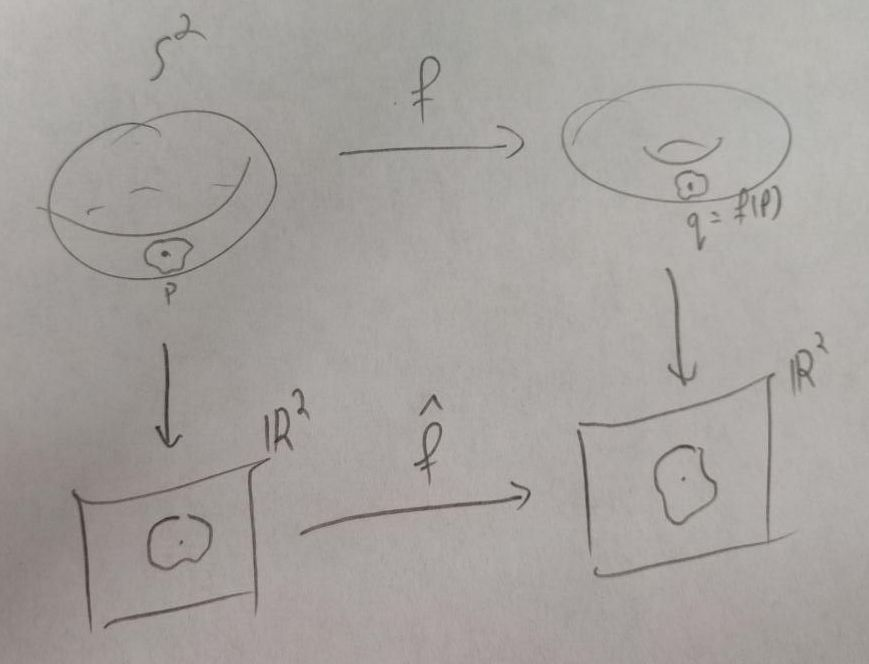
\includegraphics[width=0.8\textwidth]{sources/figure1}
\end{figure}
\\
בקורס נעסוק בהכללת משפטים מאנליזה ב־%
$\RR^n$
למשפטים על יריעות חלקות.
רוב המשפטים ניתנים להכללה ליריעות $\CCC^k$.
למשפטים מהקורס שימושים רבים בגיאומטריה, טופולוגיה, פיזיקה, אנליזה, קומבינטוריקה ואלגברה. כדי שהתיאוריה הקשורה לקורס לא תישאר באוויר נראה חלק גדול מהקורס שימושים, בעיקר בתחום של טופולוגיה דיפרנציאלית.
\\
קיימים מספר משפטים מוכרים מאנליזה.
\\
\begin{examples}
\begin{enumerate}
\item \emph{נוסחאת ניוטון-לייבניץ:}
\[\int_{\del\brs{a,b}} F = \int_{\brs{a,b}} F' \diff x\]
\item \emph{נוסחאת גרין:}
\[\int_{\del U} f\diff x + g \diff y = \iint_{U} \prs{\frac{\del g}{\del x} - \frac{\del f}{\del{y}}} \diff x \diff y\]
\item \emph{משפט גאוס:}
\[\iiint_{\Omega} \div \vec{F} \diff v = \iint_{\del \Omega} \trs{\vec{F},\vec{n}} \diff s\]
\item \emph{משפט סטוקס:}
\[\iint_{\Sigma} \trs{\rot \vec{F}, \vec{n}} \diff s = \int_{\del \Sigma} \trs{\vec{F}, \vec{\gamma}} \diff t\]
\end{enumerate}
\end{examples}
כולם נובעים ממשפט סטוקס כללי יותר אותו נוכיח בקורס.
\[\int_{\del \Omega} \omega = \int_{\Omega} \diff \omega\]

\section{דרישות קדם}
נשתמש בקורס רבות במשפט הפונקציה הסתמונה ובמשפט הפונקציה ההפוכה מ־%
$\RR^n$.
רצוי להכיר את ניסוחיהם, את המשמעויות הגיאומטריות ומספר שימושים שלהם.
נשתמש בהחלפות קואורדינטות מאלגברה לינאריות, במשפט פוביני, מטריצות יעקוביאן, במטריצות יעקוביאן, בכלל השרשרת ובמשפט קיום ויחידות של מד"ר.

\section{תרגילי בית}
בקורס יפורסמו ארבעה תרגילי בית רשמיים, רובם ברמת הבנת ההגדרות. אין חובת הגשה אך מומלץ מאוד לפתור את התרגילים כדי לוודא שאינכם הולכים לאיבוד.

\section{ציון}
הציון הסופי כולו יסתמך על הגשת עבודת בית.

\chapter{מבוא}
\section{הגדרות}
\begin{definition}
מרחב טופולוגי
$M$
נקרא
\stress{יריעה טופולוגית}
\textenglish{(topological manifold)}
אם לכל
$x \in M$
יש סביבה
$U$
שהומאומורפית לקבוצה פתוחה ב־%
$\RR^n$
עבור
$n$
כלשהו.
\end{definition}
\begin{remark}
לעתים יריעה טופולוגית כפי שהגדרנו אותה נקראת
\stress{מרחב אוקלידית לוקלית}
\textenglish{(locally Euclidean space)}.
\end{remark}
\begin{fact}
עבור יריעה טופולוגית,
$n$
קבוע מקומית.
\\
אם
$M$
קשירה,
$n$
קבוע.
\end{fact}
\begin{definition}
עבור יריעה
$M$
עם
$n$
קבוע, נגיד ש־%
$n$
הוא
\stress{המימד}
של היריעה.
\end{definition}
\begin{exercise}
מצאו אילו אותיות מבין
\textenglish{MANIFOLD}
הן יריעות. מצאו אילו הומאומורפיות.
\end{exercise}
\begin{examples}
\begin{enumerate}
\item עקומות
\item משטח ב־%
$\RR^3$
\item $S^n \subseteq \RR^{n+1}$:
נסמן
$\Uu^+ = S^n \setminus \set{p^+}$
נתאים לנקודה
$x \in \Uu^+$
על הספירה את הנקודה
$\phi^{+}(x) \in \RR^n$
המתקבלת על ידי הטלה סטרוגרפית. ראו איור
\ref{fig2}.
\begin{figure}[ht]
\centering
\caption{הטלה סטרוגרפית.}
\label{fig2}
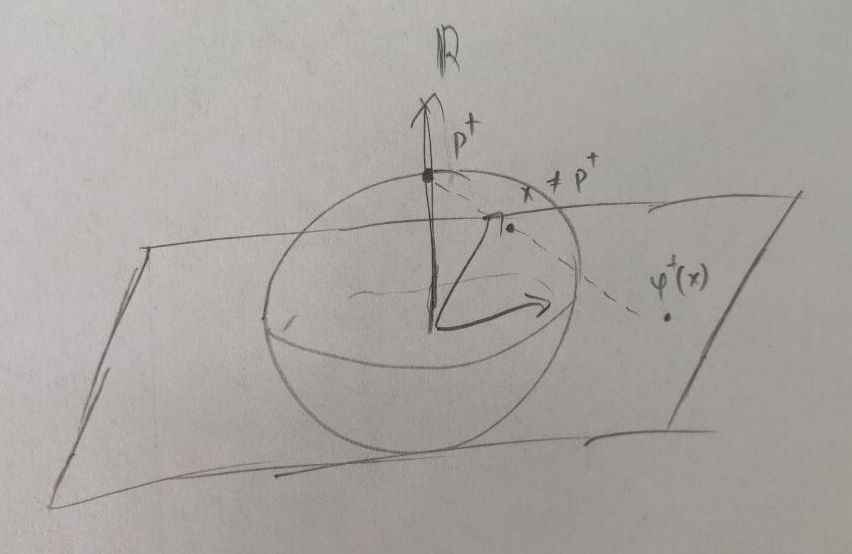
\includegraphics[width=0.8\textwidth]{sources/figure2}
\end{figure}
ניתן לראות כי
$\phi^+$
הומאומורפיזם.
אפשר באותו אופן להגדיר
$\phi^{-} \colon \U^{-} \to \RR^n$.
לכל נקודה על
$S^n$
יש סביבה הומאומורפית לקבוצה פתוחה ב־%
$\RR^n$
המתקבלת מהמקור דרך
$\phi^{\pm}$
של סביבה בתמונה, לכן
$S^n$
יריעה.
\end{enumerate}
\end{examples}
\begin{exercise}
אם
$M_1, M_2$
יריעות טופולוגיות אז
$M_1 \times M_2$
עם טופולוגיית המכפלה הינה יריעה.
אם המימד של
$M_1, M_2$
אחיד מתקיים גם
\[\text{.} \dim\prs{M_1 \times M_2} = \dim{M_1} + \dim{M_2}\]
\end{exercise}
\begin{example}
\stress{טורוס
$n$–%
מימדי} הוא
$\TT^n \ceq \prod_{k=1}^n S^1$.
ניתן להגדיר גם
$T^n = \quot{\RR^n}{\ZZ^n} = \quot{\RR^n}{\sim}$
כאשר
$x \sim y$
אם
$x-y \in \ZZ^n$.
נסמן
$\pi \colon \RR^n \to T^n$
את ההטלה הטבעית (כלומר
$\pi\prs{x} = \brs{x} = x+\ZZ^n$)
ואז
$\Uu \subseteq T^n$
פתוחה אם
$\pi^{-1}\prs{\Uu}$
פתוחה ב־%
$\RR^n$.
\end{example}
\begin{exercise}
הראו כי
$\TT^n$
הומאומורפי ל־%
$T^n$.
\end{exercise}
\begin{example}
נגדיר
\stress{מרחב פרויקטיבי הוא}
בשתי דרכים.
\begin{enumerate}[label = (\roman*)]
\item
נסתכל על ישרים דרך
$\vec{0}$
ב־%
$\RR^{n-1}$.
עבור
$\ell$
ישר דרך
$0$
נסמן
$\Uu_{\eps}\prs{\ell}$
את אוסף הישרים
$\ell'$
דרך
$\vec{0}$
כך שמתקיים
$\deg{\ell, \ell'} < \eps$.
אז קבוצה פתוחה היא איחוד כלשהו של
$\Uu_{i\in I} \Uu_{\eps_i}\prs{\ell_i}$.
\item
נגדיר גם
$\mrm{RP}^n = \quot{S^n}{\pm 1}$
כלומר
$x \sim y$
אם
$x = \pm y$.
נסמן
$\pi \colon S^n \to \mrm{RP}^n$
את ההטלה
$x \to \set{x, -x}$
ואז
$\Uu \subseteq \mrm{RP}^n$
פתוחה אם
$\pi^{-1}\prs{\Uu}$
פתוחה ב־%
$\S^n$.
\end{enumerate}
\end{example}
\begin{exercise}
הראו כי
$\mrm{RP}^n$
הומאומורפי ל־%
$\mrm{RP}^n$.
\end{exercise}
\begin{example}
$\R \mrm{P}^1$
הומאומורפי ל־%
$\S^1$.
לאחר הזיהוי מתקבל קטע המזוהה בקצותיו, וזה הומאומורפי למעגל.
\end{example}
\begin{definition}
תהי
$M$
יריעה טופולוגית.
\stress{מפה}
\textenglish{map / coordinate chart}
היא זוג
$\prs{\Uu, \phi}$
כאשר
$\Uu \subseteq M$
קבוצה פתוחה ו־%
$\phi \colon \Uu \to \phi(\Uu) \subseteq \RR^n$
הומאומורפיזם, ו־%
$\phi\prs{\Uu} \subseteq \RR^n$
פתוחה.
\end{definition}
\begin{example}
ב־%
$S^n$
הגדרנו שתי מפות
$\prs{\Uu^{\pm}, \phi^{\pm}}$.
\end{example}
\begin{definition}
תהיינה
$\prs{\Uu, \phi}, \prs{\Vv, \psi}$
מפות עבור יריעה
$M$.
אז
$\phi \circ \psi^{-1} \colon \psi\prs{\Uu \cap \Vv} \to \phi\prs{\Uu \cap \Vv}$
הומאומורפיזם שנקרא
\stress{פונקציית מעבר} \textenglish{transition map}
או
\stress{פונקציית החלפת קואורדינטות}.
ראו איור
\ref{fig3}
\begin{figure}[ht]
\centering
\caption{פונקציית מעבר.}
\label{fig3}
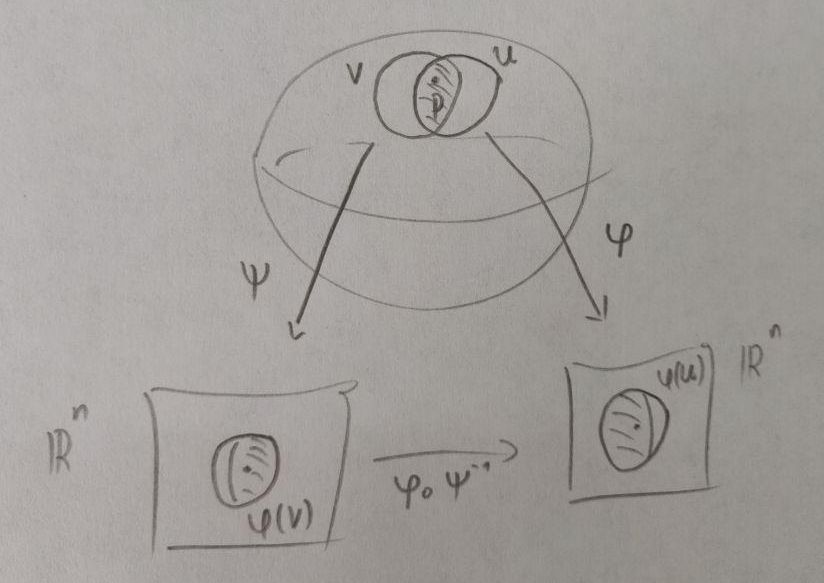
\includegraphics[width=0.8\textwidth]{sources/figure3}
\end{figure}
\end{definition}
\begin{definition}
תהי העתקה
$f \colon M \to N$
בין יריעות, ונניח בה"כ
$f\prs{\Uu_1} \subseteq \Vv_1$.
אז
$\hat{f}_1 \colon \phi_1\prs{\Uu_1} \to \psi_1\prs{\Vv_1}$
\stress{הצגה מקומית של
$f$}
(ביחס למפות
$\prs{\phi_1, \Uu_1}$
ו־%
$\prs{\psi_1, \Vv_1}$).
מתקיים
$\hat{f}_1 = \eval{\psi_1 \circ f \circ \phi_1^{-1}}{\psi_1\prs{\Uu_1}}{}$.
ראו איור
\ref{fig4}.
\begin{figure}[ht]
\centering
\caption{הצגה מקומית.}
\label{fig4}
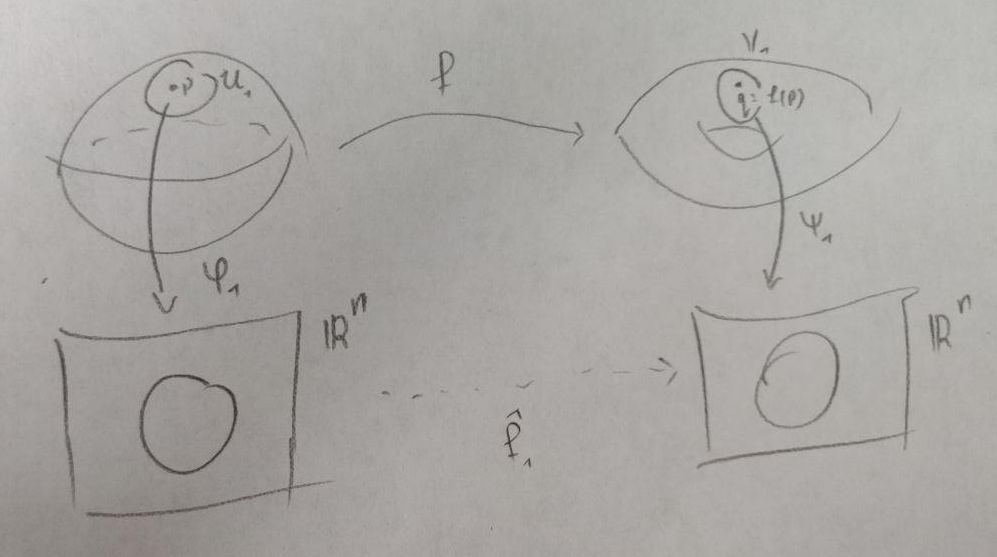
\includegraphics[width=0.8\textwidth]{sources/figure4}
\end{figure}
\end{definition}
\begin{definition}
תהיינה
$\hat{f}_1, \hat{f}_2$
שתי הצגות מקומיות של
$f \colon M \to N$.
אז
\[\text{.} \eval{\hat{f}_2}{\phi_2\prs{\Uu_1 \cap \Uu_2}}{} = \psi_2 \circ \psi_1^{-1} \circ \hat{f}_1 \circ \phi_1 \circ \phi_2^{-1}\]
כאן
$\phi_1 \circ \phi_2^{-1}$
פונקציית מעבר מ־%
$\prs{\Uu_2, \psi_2}$
ל־%
$\prs{\Uu_1, \phi_1}$
ו־%
$\psi_2 \circ \psi_1^{-1}$
פונקציית מעבר מ־%
$\prs{\Vv, \psi_1}$
ל־%
$\prs{\Vv, \psi_2}$.
ראו איור
\ref{fig5}.
\begin{figure}[ht]
\centering
\caption{פונקציית מעבר בין יריעות.}
\label{fig5}
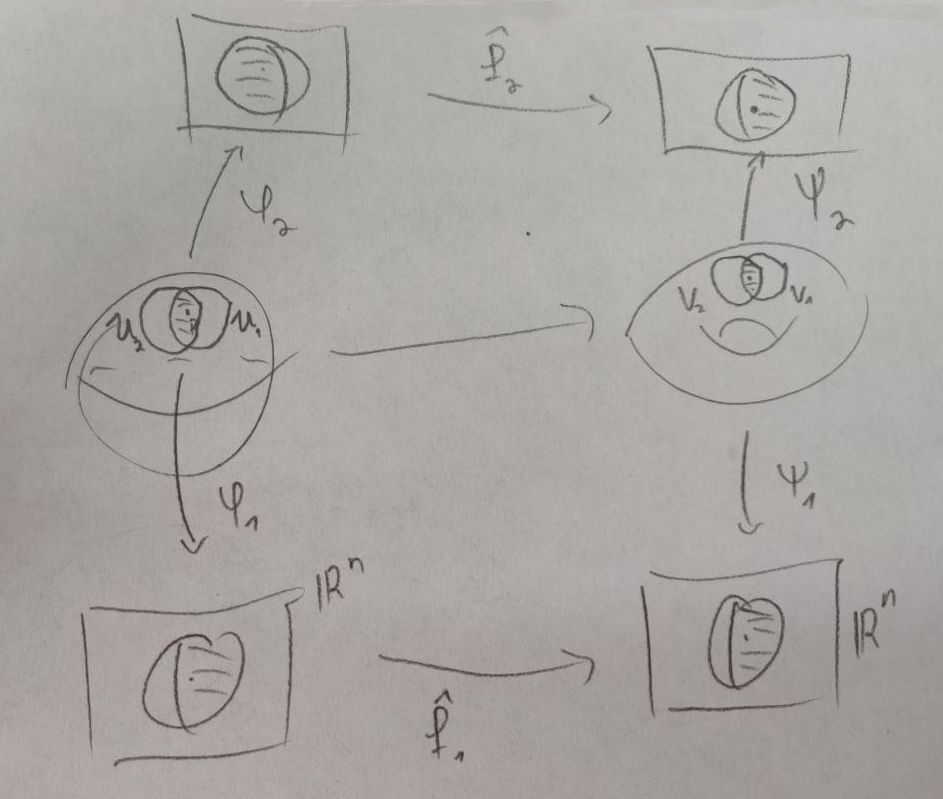
\includegraphics[width=0.8\textwidth]{sources/figure5}
\end{figure}
\end{definition}
נזכיר כי
$f \colon \Uu \to \RR^m$
עבור
$\Uu \subseteq \RR^n$
נקראת
\stress{חלקה}
\textenglish{(smooth)}
אם לכל
$x \in \Uu$
קיימות ורציפות נגזרות חלקיות של
$f$
מסדר כלשהו.
\begin{notation}
עבור
$f$
חלקה נסמן
$f \in \CCC^{\infty}$.
\end{notation}
\begin{definition}
$f \colon \Uu \to \Ww$
עבור
$\Uu \subseteq \RR^n, \Ww \subseteq \RR^m$
\stress{דיפאומורפיזם}
אם
$f$
הפיכה, ו־%
$f,f^{-1}$
חלקות.
\end{definition}
\begin{exercise}
אם
$f \colon \Uu \to \Ww$
חלקה וגם
$\Uu \subseteq \RR^n, \Ww \subseteq \RR^m$
אז
$m=n$.
\end{exercise}
\begin{examples}
\item $f(x) \ceq \fcases{0 & x < 0 \\ x^2 & x \geq 0}$
איננה חלקה.
\item $f(x) \ceq \fcases{0 & x \leq 0 \\ e^{-\frac{1}{x}} & x > 0}$
חלקה (אך איננה אנליטית).
\item נגדיר $\Uu = \prs{-\frac{\pi}{2}, \frac{\pi}{2}}, \Ww = \R$.
אז
$\tan \colon \Uu \to \Ww$
דיפאומורפיזם.
\end{examples}
\begin{exercise}
\begin{enumerate}
\item אם
$F$
דיפאו' גם
$F^{-1}$
דיפאו'.
\item הרכבה של דיפאו' היא דיפאו'.
\item אם
$F_1 \colon \Uu_1 \to \Ww_1$
ו־%
$F_2 \colon \Uu_2 \to \Ww_2$
דיפאו' אז
$F_1 \times F_2 \colon \Uu_1 \times \Uu_2 \to \Ww_1 \to \Ww_2$
דיפאו'.
\item אם
$-\infty \leq a \leq b \leq \infty$
ו־%
$-\infty \leq c \leq d \leq \infty$
אז
$\prs{a,b}$
דיפאומורפי ל־%
$\prs{c,d}$.
\item הקבוצות במישור
מאיור
\ref{fig6}
דיפאומורפיות.
\begin{figure}[ht]
\centering
\caption{קבוצות דיפאומורפיות במישור.}
\label{fig6}
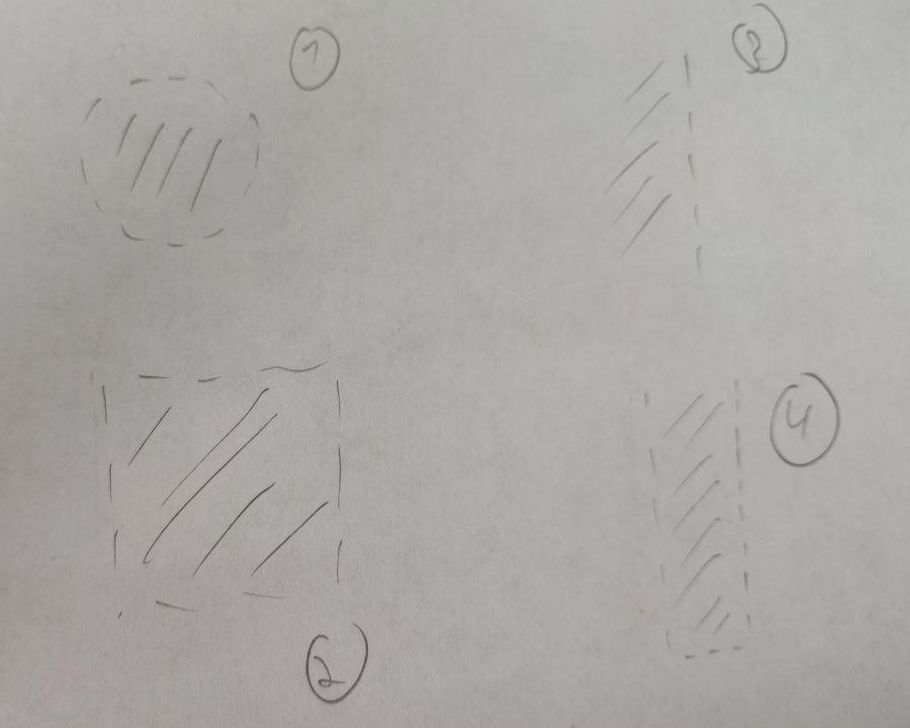
\includegraphics[width=0.8\textwidth]{sources/figure6}
\end{figure}
\end{enumerate}
\end{exercise}
\section{מבנה חלק}
נרצה להגדיר מתי העתקה
$f \colon M \to \RR$
הינה גזירה/חלקה בנקודה
$p$.
ננסה להגדיר גזירות של העתקה
$f$
כנ"ל.
\begin{description}
\item["הגדרה":]
\emph{$f$
גזירה ב־%
$p \in M$
אם כל הצגה מקומית
$\hat{f}$
גזירה ב־%
$\phi\prs{p}$.}
הגדרה זאת איננה טובה כי בהינתן שתי הצגות מקומיות סביב
$p$
ופונקציית מעבר
$\psi$,
$\hat{f}_1 = \hat{f}_2 \circ \psi$
איננה בהכרח גזירה.

\item["הגדרה 2":]
נניח כי
$M \subseteq \RR^n$
יריעה. נאמר כי
$f \colon M \to \RR$
חלקה אם ניתן להרחיב את
$f$
לפונקציה חלקה
$f \colon \Uu \to \RR$
כאשר
$\Uu$
סביבה פתוחה של
$M$.
\\
גם בהגדרה זו יש בעיות, כפי שנראה מיד בדוגמה.
\end{description}
\begin{example}
ניקח
$M = \RR \subseteq \RR$.
נסתכל על שלוש מפות
$\prs{\Uu_i, \phi_i}, i \in [3]$
כאשר
$\Uu_i = \RR$
והמפות מוגדרות על ידי
\begin{align*}
\phi_1(x) &= x \\
\phi_2(x) &= x^3 \\
\text{.} \phi_3(x) &= \sqrt[3]{x}
\end{align*}
תהי
$f(x) = \sum_{i=0}^{\infty} a_i x^i$.
אז
$\hat{f}_1 = f$
ונקבל כי מה"הגדרה"
$\hat{f}_1$
חלקה אם ורק אם
$f$
חלקה במובן של אינפי.
נקבל
\[\hat{f}_2(u) = f\circ \phi_2^{-1}(u) = \sum_{i=0}^{\infty} a_i \cdot u^{\frac{i}{3}}\]
לכן תנאי הכרחי עבור חלקות של
$\hat{f}_2$
הוא ש־%
$a_i = 0$
לכל
$i \not\equiv 0 \mod{3}$.
נקבל באותו אופן
\[\hat{f}_3\prs{w} = \sum_{i=1}^{\infty} a_i w^{3i}\]
ונקבל פחות הצגות חלקות מאשר בהצגה המקומית הראשונה.
\end{example}
\begin{example}
נגדיר
$M_1 = \set{\prs{x,y} \in \RR^2}{y=0}$
ו־%
$M_2 = \set{\prs{x,y} \in \RR^2}{y=\abs{x}}$.
נגדיר העתקה
$P \colon M_2 \to M_1$
ע"י
$\prs{x,\abs{x}} \mapsto \prs{x,0}$.
זהו הומיאומורפיזם.
\begin{exercise}
$f_1 \colon M_1 \to \RR$
ע"י
$\prs{x,0} \mapsto \phi\prs{x}$
חלקה אם ורק אם
$\phi$
חלקה כפונקציה
$\RR \to \RR$.
\end{exercise}
\begin{exercise}
$f_2\prs{x, \abs{x}} = \abs{x}$
פונקצייה חלקה
$M_2 \to \RR$.\\
רמז: ניתן להרחיב אותה לפונקציה
$f_2\prs{x,y} = y$
כאשר
$f_2 \colon \RR^2 \to \RR$.
\end{exercise}
כאשר נפעיל את הזיהוי בין
$M_1$
ל־%
$M_2$
על ידי
$P$
נקבל כי
$f_2$
פונקצייה חלקה!
לכן ה"הגדרה" תלויה בשיכון
$M \rmono \RR^n$
ולא רק ביריעה עצמה.
\end{example}
נתקלנו בבעייה. המבנה של יריעה טופולוגית הינו חלש מידי ונראה שאין סיכוי להגדיר עליו נגזרת. איך נעקוף זאת?
נרצה לדרוש שההעתקות המעבר יהיו חלקות, ואז
$\hat{f}_1 = \psi \circ \hat{f}_2 \circ \phi$
תהיה גזירה אם ורק אם
$\hat{f}_2$
גזירה, עבור
$\psi, \phi$
העתקות מעבר.\\
\begin{definition}
תהי
$M$
יריעה. מפות
$\prs{\Uu, \phi}, \prs{\Vv, \psi}$
יקראו
\stress{מתואמות}
(\textenglish{compatible})
אם
$\psi \circ \phi^{-1}, \phi \circ \psi^{-1}$
חלקות (כלומר, דיפאומורפיזמים).
\end{definition}
\begin{exercise}
תהי
$f \colon \Uu \cap \Vv \to \RR$.
אז
$f \circ \phi^{-1}$
חלקה אם ורק אם
$f \circ \psi^{-1}$
חלקה, כאשר
$\phi,\psi$
מתואמות.
\end{exercise}
\begin{definition}
תהי
$M$
יריעה.
\stress{אטלס חלק}
\textenglish{(smooth atlas / $\CCC^{\infty}$ atlas)}
על
$M$
הוא משפחת מפות מתואמות
$\set{\prs{\Uu_{\alpha}, \phi_{\alpha}}}_{\alpha \in I}$
כך שמתקיים
$M = \bigcup_{\alpha \in I} \Uu_{\alpha}$.
\end{definition}
\begin{example}
ניקח
$M = S^1$
ואז
$\set{\prs{\Uu^{\pm}, \phi^{\pm}}}$
שהגדרנו קודם הינו אטלס.
\end{example}
\begin{claim}
האטלס הנ"ל הינו חלק.
\end{claim}
\begin{proof}
\begin{figure}[h!]
\caption{the stereographic map.}
\label{stereographic}
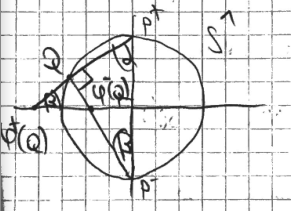
\includegraphics[scale=1]{sources/stereographic}
\end{figure}
מתקיים
\[\text{.} \Uu^+ \cap \Uu^- = S^1 \setminus \set{p^+, p^-}\]
כמובן
$\phi^{\pm}\prs{\Uu^+ \cap \Uu^-} = \RR \setminus \set{0}$.
ראו איור
\ref{stereographic}.
מתקיים
$\phi^-\prs{Q} = \tan\prs{\beta}$
וגם
$\phi^+\prs{Q} = \frac{1}{\tan\prs{\beta}}$.
לכן אם
$x = \phi^+\prs{Q}$
נקבל
$\phi^- \circ \prs{\phi^+}^{-1}\prs{x} = \frac{1}{x}$
פונקציית מעבר חלקה.
כנ"ל לפונקציית המעבר לכיוון השני, לכן האטלס חלק.
\end{proof}
\begin{definition}
שני אטלסים חלקים נקראים
\stress{שקולים}
אם האיחוד שלהם הוא אטלס חלק.
\end{definition}
\begin{exercise}
שקילות זאת הינה אכן יחס שקילות בין אטלסים חלקים על
$M$.
\end{exercise}
\begin{definition}
\stress{מבנה חלק}
על
$M$
זו מחלקת שקילות של אטלסים.
\end{definition}
\begin{example}
ניקח
$M = \RR$
עם
$\Uu_i = \RR$
וההעתקות
$\phi_1 = \id, \phi_2 = x^2, \phi_3 = \sqrt[3]{x}$.
אז שלושת האטלסים
$\set{\prs{\Uu_i, \phi_i}}$
אטלסים לא מתואמים בזוגות ולכן מייצגים שלושה מבנים חלקים שונים.
\end{example}
\begin{definition}
תהי
$\prs{M,\mcal{A}}$
יריעה עם אטלס חלק.
נגדיר
$f \colon M \to \RR$
\stress{גזירה}
בנקודה
$p \in M$
אם
$\hat{f} \colon \phi\prs{\Uu} \to \RR$
גזירה ב־%
$\phi\prs{p}$
עבור
$\prs{\Uu, \phi}$
מפה סביבה
$p$
מהאטלס
$\mcal{A}$.
\end{definition}
\begin{exercise}
בדקו כי הנ"ל מוגדר היטב.
\end{exercise}
\begin{definition}
\stress{יריעה חלקה}
היא יריעה טופולוגית
$M$
עם בחירה של אטלס חלק על
$M$.
\end{definition}
\begin{claim}
בכל מחלקת שקילות של אטלסים קיים אטלס מקסימלי.
\end{claim}
\begin{corollary}
בחירת מבנה חלק שקולה לבחירת אטלס חלק מקסימלי על
$M$.
\end{corollary}
\begin{definition}
תהיינה
$\prs{N, \Aa_N}, \prs{M, \Aa_M}$
שתי יריעות חלקות ותהי
$f \colon M \to N$.
אז
$f$
תיקרא
\stress{גזירה}
ב־%
$p \in M$
אם
$\hat{f} = \psi \circ f \circ \phi^{-1}$
גזירה ב־%
$\phi\prs{p}$,
ההצגה המקומית ביחס למפות
$\prs{\Uu, \phi} \in \Aa_M, p \in \Uu$
ו־%
$\prs{\Vv, \psi} \in \Aa_N, f\prs{p} \in \Vv$.
\end{definition}
\begin{exercise}
בדקו כי הנ"ל מוגדר היטב ביחס למפות מתואמות.
\end{exercise}
\begin{definition}
פונקציה
$f \colon M \to N$
\stress{חלקה}
אם כל ההצגות המקומיות של
$f$
ביחס למפות מתואמות הן פונקציות חלקות.%
\newlecture{28 באוקטובר}%
{2018}
\end{definition}
\begin{remark}
כדי לבדוק חלקות, די לבדוק חלקות של פונקציות מתואמות עם מפות שמכסות את היריעה.
\end{remark}
\begin{definition}
פונקציה הפיכה
$f$
כאשר
$f,f^{-1}$
חלקות נקראת
\stress{דיפאומורפיזם}.
\end{definition}
\begin{exercise}
אם
$f \colon M \to N$
דיפאומורפיזם, אז
$\dim M = \dim N$.
\end{exercise}
\begin{exercise}
דיפאומורפיזמים שומרים על פונקציות חלקות.
אם בדיאגרמה הבאה
$\phi,\psi$
איזומורפיזמים, אז
$h$
חלקה אם ורק אם
$h'$
חלקה.
\[
\begin{tikzcd}
M \arrow[r,"h"] \arrow[d,"\phi"] & N \arrow[d,"\psi"] \\
M' \arrow[r, dotted, "h'"] & N'
\end{tikzcd}
\]
\end{exercise}
\begin{definition}
\stress{יריעה דיפרנציאבילית
$\CCC^r$}
היא יריעה טופולוגית עם אטלס בו פונקציות המעבר חלקות
$\CCC^r$.
\end{definition}
\begin{exercise}
תהי
$\prs{M,\Aa}$
יריעה חלקה ותהי
$\prs{\Uu, \phi}$
מפה מתואמת עם
$\Aa$.
אז
$\phi \colon \Uu \to \phi\prs{\Uu} \subseteq \RR^m$
דיפאומורפיזם.
\end{exercise}
\begin{example}
תהי
$M = \RR$
עם
$\Aa_1 = \set{\prs{\RR,\1}}$
המבנה החלק הסטנדרטי, ועם
$\Aa_2 = \set{\prs{\RR,x^3}}$.
אז
$\prs{M,\Aa_1}, \prs{M,\Aa_2}$
יריעות חלקות שונות, אך דיפאומורפיות.
נסמן
$f(x) = \sqrt[3]{x}$.
אז
$\hat{f} = \1_{\RR}$
ולכן
$f$
דיפאומורפיזם. ראה איור
\ref{diffeo}.
\begin{figure}[h!]
\centering
\caption{דיפאומורפיזם.}
\label{diffeo}
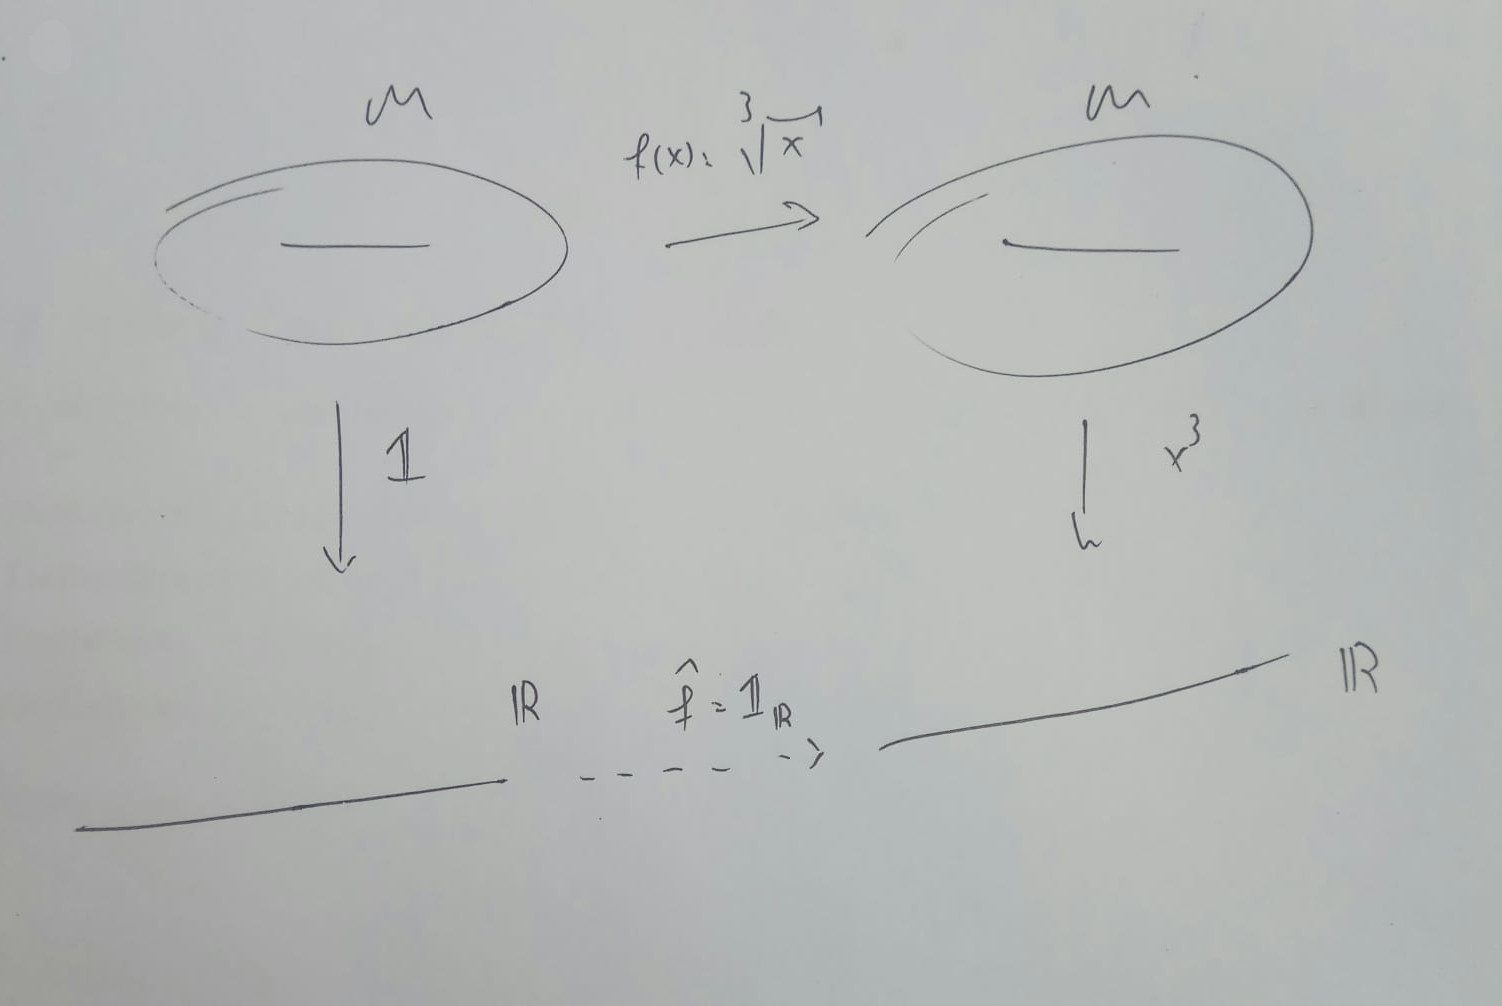
\includegraphics[scale=0.6]{sources/diffeo}
\end{figure}
\end{example}
\begin{question}
האם קיימים מבנים שאינם דיפאומורפיים על אותה יריעה טופולוגית?
עבור
$\dim M \leq 3$
התשובה נכונה.
עבור
$\dim M = 1$
נסו
\textbf{כתרגיל}.
עבור
$\dim M \geq 4$
הדבר תלוי ביריעה.
\end{question}
\begin{example}
בטבלה
\ref{sphere_diffeo}
מספר המבנים הדיפאומורפיים של הספירה.
עבור
$n=4$
זאת בעייה פתוחה הנקראת
\textenglish{smooth Poincaré conjecture}.
\begin{figure}[h!]
\caption{מבנים דיפאומורפיים של הספירה.}
\label{sphere_diffeo}
\centering
\begin{tabular}{|c|c|}
\hline $n$ & מספר מבנים חלקים שונים של $S^n$ עד כדי דיפאומורפיזם \\
\hline $1$ & $1$ \\
\hline $2$ & $1$ \\
\hline $3$ & $1$ \\
\hline $4$ & ? \\
\hline $5$ & $1$ \\
\hline $6$ & $1$ \\
\hline $7$ & $28$ \\
\hline $8$ & $2$ \\
\hline $9$ & $8$ \\
\hline $10$ & $6$ \\
\hline $11$ & $992$ \\
\hline $12$ & $1$ \\
\hline
\end{tabular}
\end{figure}
\end{example}
\begin{example}
ב־%
$\RR^n$
יש מבנה דיפאומורפי אחד לכל
$n \neq 4$,
ואינסוף עבור
$n=4$.
\end{example}
\section{תתי־יריעות}
\begin{definition}
תהי
$M$
יריעה טופולוגית
ממימד
$m$
ותהי
$N \subseteq M$
עם הטופולוגיה המושרית.
$N$
תיקרא
\stress{תת־יריעה טופולוגית}
אם לכל
$x \in N$
קיימת מפה
$\prs{\Uu,\phi}$
של
$M$
עם
$x \in \Uu$
וגם
$\phi^{-1}\prs{\RR^n} = \Uu \cap N$.
(כאן
$\RR^n = \set{\prs{x_1, \ldots, x_n, 0, \ldots, 0}} \subseteq \RR^m$)
\end{definition}
\begin{examples}
\begin{itemize}
\item $W \subseteq M$
קבוצה פתוחה היא תת־יריעה חלקה.
\item אם
$F \colon \RR^m \to \RR^n$
אז הגרף של
$F$,
\[\gr\prs{F} = \set{\prs{x,F(x)}}{x \in \RR^m} \subseteq \RR^m \times \RR^n\]
היא תת־יריעה.
אם
$F$
רציפה זאת רק תת־יריעה טופולוגית, אם
$F$
חלקה זאת תת־יריעה חלקה, וכו'.
תהי
$\Uu \subseteq \RR^m$
פתוחה. אז
$\Uu \times \RR^n$
פתוחה במרחב
$\RR^m \times \RR^n$.
נגדיר
\begin{align*}
\phi_{\Uu} \colon \Uu \times \RR^n &\to \Uu \times \RR^n \subseteq \RR^m \times \Rr^n \\
\prs{x,y} &\mapsto \prs{x,y-F(x)}
\end{align*}
ואז
$\gr\prs{F} \cap \prs{\Uu \cap \RR^n} \stackrel{\sim}{\longleftrightarrow} \Uu \times \set{0}$
המפה שנדרשת בהגדרה.
אם
$F$
רציפה,
$\phi_{\Uu}$
הומאומורפיזם ולכן זאת תת־יריעה טופולוגית.
אם
$F$
חלקה,
$\phi_{\Uu}$
חלקה, כלומר מתואמת עם האטלס הסטנדרטי, וזאת תת־יריעה חלקה.
\end{itemize}
\end{examples}
\begin{exercise}
גרף של
$\abs{x}$
הוא תת־יריעה טופולוגית אך לא חלקה.
\end{exercise}
\begin{exercise}\label{submanifold}
תת־יריעה טופולוגית היא יריעה טופולוגית.
\end{exercise}
\begin{proposition}
תהי
$N^n \subseteq M^m$
(כלומר
$N$
ממימד
$n$,
$M$
ממימד
$m$)
תת־יריעה חלקה. אזי
$M$
משרה על
$N$
מבנה של יריעה חלקה.
\end{proposition}
\begin{proof}
מתרגיל
\ref{submanifold}
תת־יריעה היא יריעה טופולוגית. נשאר להראות כי
$M$
משרה מבנה חלק.\\
ניקח
$\set{\prs{\Uu_x,\phi_x}}_{x \in N}$
מפות מההגדרה של תת־יריעה חלקה ונגדיר
\[\mcal{A} = \set{\prs{\Uu_x \cap N, \rest{\phi_x}{\Uu_x \cap N}}}_{x \in N}\]
אטלס שמכסה את
$N$.
נשאר להראות כי המפות מתואמות.
$\prs{\Uu_x, \phi_x}$
ו־%
$\prs{\Uu_y, \phi_y}$
מתואמות, לכן פונקציות המעבר
\[\phi_y \circ \phi_x^{-1} \colon \phi_x\prs{\Uu_x \cap \Uu_y} \to \phi_y\prs{\Uu_x \cap \Uu_y}\]
חלקות.
לכן הצמצום באטלס
$\mcal{A}$,
שהינו
\[\rest{\phi_y \circ \phi_x^{-1}}{\RR^n \cap \phi_x\prs{\Uu_x \cap \Uu_y}} \colon \RR^n \cap \phi_x\prs{\Uu_x \cap \Uu_y} \to \RR^n \cap \phi_y\prs{\Uu_x \cap \Uu_y}\]
גם הוא חלק.
\end{proof}
\begin{example}
נתונה מערכת משוואות
\[\fcases{F_1\prs{x_1, \ldots, x_m} = 0 \\
\vdots \\
F_r\prs{x_1, \ldots, x_m} = 0}\]
כאשר
$F_i$
חלקות. נניח שבנקודה
$\vec{x}$
כך ש־%
$\vec{F}\prs{\vec{x}} = 0$
מתקיים
$\rank\prs{\frac{\del \vec{F}}{\del \vec{x}}} = r$
(הדרגה מקסימלית).
ממשפט הפונקציה הסתומה ניתן לבודד
$m-r$
קואורדינטות
$\vec{x}''$
כאשר
$\vec{x}'$
שאר הקואורדינטות.
נסמן
$\vec{x} = \prs{\vec{x}'',\vec{x}'}$
בה"כ ואז לוקלית ליד
$\vec{x}$
קבוצת הפתרונות
$\vec{F}\prs{\vec{x}} = \vec{0}$
נראית כמו גרף של פונקצייה
\begin{align*}
G \colon \RR^{m-r} &\to \RR^n \\
\text{.} \phantom{G \colon \RR^{m}} x'' &\mapsto G\prs{x''} \subseteq \RR^r
\end{align*}
\end{example}
\begin{example}
עבור
$F\prs{x_1, x_2} = x_1^2 + x_2^1 - 1$,
מתקיים
$\frac{\del F}{\del x} = \prs{2x_1, 2x_2}$.
כאשר
$x_1, x_2 \neq 0$
ניתן להציג את
$x_1$
כפונקציה של
$x_2$
או להיפך.
לוקלית, ליד
$x$,
$M = \set{x}{F(x) = 0}$
היא יריעה חלקה.
אם תנאי של משפט הפונקציה הסתומנה מתקיים לכל
$x \in M$,
אז
$M$
יריעה חלקה (גלובלית).
\end{example}
\begin{exercise}
עבור תת־יריעה כמו בדוגמה, מתקיים
$\dim M = m-r$.
\end{exercise}
\begin{theorem}
נניח ש־%
$N \subseteq \RR^m$
תת־קבוצה כך שלכל
$x \in N$
קיימת סביבה
$\Uu \subseteq \RR^m$
ו־%
$r = m-n$
פונקציות חלקות
$F_i \colon \Uu \to \RR^m$
(עם
$r$
קבוע עבור
$N$)
כך שמתקיימים התנאים הבאים.
\begin{align*}
N \cap \Uu = \set{\vec{x} \in \Uu}{\vec{f}\prs{\vec{x}} = \vec{0}} \\
\rank\prs{\frac{\del \vec{F}}{\del\vec{x}}} = r
\end{align*}
אז
$N \subseteq \RR^m$
תת־יריעה ממימד
$n = m-r$.
\end{theorem}
\begin{remark}
הכיוון ההפוך איננו בהכרח נכון.
אם
$\set{\vec{x} \in \RR^n}{\vec{F}\prs{\vec{x}} = 0}$
תת־יריעה של
$\RR^m$,
ייתכן ש־%
$\vec{F}$
איננה מקיימת את תנאי משפט הפונקציה הסתומה.
המשפט הינו תנאי מספיק שאינו הכרחי.
\end{remark}
\begin{examples}
\begin{itemize}
\item $S^n$
קבוצת הפתרונות של
\[\text{.} F\prs{x_1, \ldots, x_{n+1}} = \sum_{i=1}^{n+1} x_i^2 - 1\]
מתקיים
$\prs{\frac{\del F}{\del x_i}} = \prs{2x_1, 2x_2, \ldots, 2x_{n+1}}$
ולכן
לכל
$\vec{x} \neq \vec{0}$
הדרגה היא
$1$.
$\vec{0}$
לא ביריעה, לכן זאת יריעה
$n$%
־מימדית.
\item (\textbf{תרגיל})
תהי
$B\prs{x}$
תבנית ריבועית שאיננה מנוונת.
$N = \set{x}{B(x) = 1}$
תת־יריעה.
$\set{x}{B(x) = 0}$
איננה בהכרח תת־יריעה, לדוגמה עבור
$x_1^2 + x_2^2 - x_3^2$
מתקבל חרוט דו־צדדי שאיננו תת־יריעה.
\item $\mrm{SL}\prs{n,\RR} \subseteq M_{n\times n}\prs{\RR}$
תת־יריעה כאשר
$M_{n\times n}\prs{\RR}$
מזוהה עם
$\RR^{n^2}$
עם המבנה החלק הסנדרטי.
\begin{proof}
תהי
\begin{align*}
F \colon M_{n\times n} &\to \RR \\
A &\to \det A
\end{align*}
ואז
$\mrm{SL}_n = \set{A}{FA = 1}$.
תהיינה
$\prs{x_{i,j}}_{i,j=1}^n$
קואורדינטות של
$M_{n\times n}$.
צריך להוכיח שלכל
$\vec{x} \in \mrm{SL}_n$
מתקיים
$\prs{\frac{\del F}{\del x_{i,j}}} \neq \vec{0}$,
כלומר שקיים
$x_{i,j}$
כך ש־%
$\frac{\del F}{\del x_{i,j}} \neq 0$.
נחשב.
\begin{align*}
\frac{\del F}{\del x_{i,j}} \prs{A} &= \rest{\frac{\diff}{\diff t}}{t=0} \prs{\det \prs{A + t\cdot T_{i,j}}} \\ &= \rest{\frac{\diff}{\diff t}}{t=0}\prs{\det A \cdot \det\prs{\1 + tA^{-1}T_{i,j}}} \\
&= \det A \cdot \frac{\diff}{\diff t}\prs{\det \prs{\1 + tA^{-1} T_{i,j}}} \\
&= \det A \cdot \tr \prs{A^{-1} T_{i,j}}
\end{align*}
כאשר
$\prs{T_{i,j}}_{k,l} = \delta_{k,i} \delta_{j,l}$
וכאשר
$\det\prs{1+\eps B} = 1 + \eps \tr B + O\prs{\eps^2}$
נובע מפיתוח לפי תמורות.
מתקיים
$A^{-1} = \prs{\frac{M_{i,j}}{\abs{A}}_{i,j}}$
מנוסחה עם מינורים.
מתקיים כי
$B T_{i,j}$
שווה למטריצה עם העמודה
$C_i\prs{B}$
ה־%
$i$
של
$B$
בעמודה ה־%
$j$,
ואפסים בשאר המקומות.
לכן
\[\prs{A^{-1}T_{i,j}}_{l,k} = \frac{M_{k,l}}{\abs{A}}\]
ולכן
קיבלנו
\[\text{.}\frac{\del F}{\del x_{i,j}}\prs{A} = \det A \cdot \frac{M_{j,i}}{\abs{A}} = M_{i,j}\]
$A$
הפיכה ולכן לא כל המינורים מתאפסים ונקבל כי
$\prs{\frac{\del F}{\del x_{i,j}}} \neq \vec{0}$.
לכן גם
$\dim \mrm{SL}\prs{n,\RR} = n^2 - 1$.
\end{proof}
\item \begin{exercise}
$O\prs{n} \leq M_{n\times n}$
תת יריעה.
\end{exercise}
\item $\TT^n \subseteq \RR^{2n}$
כאשר
$\TT^n \cong \prs{S^1}^n$
ו־%
$\RR^{2n} \cong \prs{\RR^2}^n$,
ניתן להצגה ע"י המשוואות
$x_{2k-1}^2 + x_{2k}^2 - 1 = 0$
כאשר
$k \in \brs{n}$.
עבור
$\TT^2$,
ניתן לכתוב
\[\text{.} F\prs{x_1, x_2, x_3} = \prs{\sqrt{x_1^2 + x_2^2} - 2}^2 + x_3^2 - 1 = 0\]
\end{itemize}
\end{examples}
\begin{exercise}
$\nabla F \neq \vec{0}$
בנקודה
$x \in \TT^2$.
\end{exercise}
\begin{exercise}
ניקח $\TT^2 = \quot{\RR^2}{\ZZ^2}$
ונגדיר
\[\fcases{\phi_1(t) = \phi_1(0) + v_1 t \\
\phi_2\prs{t} = \phi_2(0) + v_2 t}\]
תנועה חופשית של חלקיק ב־%
$\TT^2$.
לאילו
$v_i$
המסלול הוא תת־יריעה של
$\TT^2$?
\end{exercise}
\begin{example}
תהי
$f \colon M \to N$
חלקה.
אזי
\[\gr\prs{f} = \set{\prs{x,f(x)}}{x \in M} \subseteq M \times N\]
תת־יריעה.
\stress{האלכסון}
הוא
$\Delta \subseteq M \times M$
הגרף של
$\1_{M}$.
הכייון ההפוך איננו נכון. אם
$\gr{f}$
תת־יריעה, לא מובטח כי
$f$
חלקה.
\end{example}
\begin{remark}
ברוב הדוגמאות, יריעות הן תתי־יריעות של
$\RR^N$.
\end{remark}
\begin{theorem}[\textenglish{Whitney}]
כל יריעה
$M^m$
ניתנת לשיכון כת־יריעה חלקה ב־%
$\RR^N$
עבור
$N$
מסוים.
\end{theorem}
\begin{remark}
המקרה האופטימלי הכללי הוא
$N=2m$.
ל־%
$2m-1$
אין תמיד שיכון כתת־יריעה חלקה.
$\RR\mrm{P}^2, K^2$
לא ניתנים לשיכון ב־%
$\RR^3$.
\end{remark}
\begin{exercise}
תהי $N \subseteq \RR^m$
תת־יריעה ויהי
$x \in N$.
$f \colon N \to \RR$
חלקה ליד
$x$
אם ורק אם ניתן להרחיב את
$f$
לפונקציה
$F \colon \Uu \subseteq \RR^m \to \RR$
חלקה, כאשר
$\Uu$
סביבה של
$x$
ב־%
$\RR^m$.
\end{exercise}
\section{נגזרות}
\begin{definition}
תהי
$M$
יריעה חלקה.
\stress{עקומה}
$\gamma$
היא העתקה
$\gamma \colon \prs{a,b} \to M$
חלקה (ביחס למבנה החלק של
$M$
והסטנדרטי ב־%
$\RR$).
\end{definition}
\begin{question}
מהי
$\dot{\gamma}(x)$,
"וקטור המהירות של חלקיק הנע לאורך
$\gamma$"?
אם
$M \subseteq \RR^n$
\textbf{עם שיכון נתון}
נוכל להסתכל על
$\vec{\gamma} = \pmat{\gamma_1\prs{t} \\ \vdots \\ \gamma_n\prs{t}}$
ואז לגזור
$\dot{\gamma}(x) = \pmat{\dot{\gamma}_1\prs{t} \\ \vdots \\ \dot{\gamma}_n\prs{t}}$
וקטור שמשיק ל־%
$M$
בנקודה
$\gamma\prs{x}$.
\end{question}
\begin{remark}
תהי
$M$
יריעה חלקה.
היינו רוצים להגדיר מרחב משיק בנקודה
$p$
להיות אוסף וקטורי המהירות של מסילות העוברות דרך
$p$.
אין לנו דרך טובה להגדיר וקטורי מהירות באופן כללי, לכן צריך לעקוף זאת.
\end{remark}
\begin{definition}
תהיינה
$\gamma_i \colon \prs{-\eps, \eps} \to M$
מסילות עבור
$i \in [2]$
וכאשר
$\gamma_i(0) = p$.
אזי
$\gamma_1 \sim \gamma_2$
אם קיימת מפה
$\prs{\Uu, \phi}$
סביב
$p$
כך שלהצגות המקומיות
$\hat{\gamma}_i = \phi \circ \gamma_i$
אותו וקטור מהירות
$\dot{\hat{\gamma}}_1(0) = \dot{\hat{\gamma}}_2(0)$.
\end{definition}
\begin{definition}
\stress{וקטור משיק בנקודה
$p$}
הוא מחלקת שקילות של עקומות
$\bar{\gamma}$
עם
$\gamma(0) = p$.
\end{definition}
\begin{exercise}
הראו כי שקילות עקומות בהגדרה הנ"ל היא אכן יחס שקילות.
\end{exercise}
\begin{remark}
יחס השקילות
$\sim$
אינו תלוי בבחירת המפה סביב
$p$.
נסתכל על שתי מפות
$\phi, \psi$
ואז
\[\underset{\hat{\gamma}_i}{\underbrace{\phi \circ \gamma_i}} = \prs{\phi \circ \psi^{-1}} \circ \underset{\hat{\hat{\gamma}}_i}{\underbrace{\psi \circ \gamma_i}}\]
ומכלל השרשרת
\[\dot{{\hat{\gamma}}}_i(0) = \rest{D\prs{\phi \circ \psi^{-1}}}{\phi\prs{p}} \cdot \dot{{\hat{\hat{\gamma}}}}_i(0)\]
ואז
\[\text{.} \dot{\hat{\hat{\gamma}}}_1 = \dot{\hat{\hat{\gamma}}}_2 \iff \dot{{\hat{\gamma}}}_1 = \dot{\hat{{\gamma}}}_2\]
\end{remark}
\begin{definition}
נגדיר
\[T_p M = \quot{\set{\text{smooth paths $\gamma(0)=p$}}}{\sim}\]
\stress{המרחב המשיק בנקודה
$p \in M$}.
\end{definition}

\begin{remark}
$\phi \colon M \to \RR^m$
מגדירה העתקה

\begin{align*}
D\phi_p \colon T_p M &\to \RR^m \\
\brs{\gamma\prs{t}} &\to \dot{\prs{\phi \circ \gamma}}(0)
\end{align*}

\end{remark}
\begin{exercise}
\begin{enumerate}
\item \[D \phi_p \colon T_p M \to \RR^m\]
חח"ע ועל.
\item בהינתן שתי מפות
$\prs{\Uu,\phi}$, $\prs{\Vv,\psi}$
סביב
$p$,
הדיאגרמה הבאה קומוטטיבית.
\[
\begin{tikzcd}
& T_p M \arrow[dl, swap, "D \phi_p"] \arrow[dr, "D \psi_p"] \\
\RR^m \arrow[rr, swap, dashed, "\rest{D\prs{\psi \circ \phi^{-1}}}{\phi(p)}"] & & \RR^m
\end{tikzcd}
\]
\item
ל־%
$T_p M$
יש מבנה לינארי טבעי, ע"י משיכת המבנה הלינארי מ־%
$\RR^m$.
נגדיר
\begin{align*}
\fcases{ \sigma + \eta \ceq D\phi_p^{-1} \prs{D \phi_p\prs{\sigma} + D\phi_p\prs{\eta}} \\
c \cdot \sigma \ceq D\phi_p^{-1} \prs{c \cdot D\phi_p\prs{\sigma}}
}
\end{align*}
ונשאיר כתרגיל בדיקה כי הדבר אינו תלוי בבחירת המפה
$\phi$.
(זה נובע מכך שהעתקות המעבר הינן לינאריות)
\end{enumerate}
\end{exercise}
\begin{example}
תהי
$\Uu \subseteq \RR^n$
פתוחה וניקח את המפה
$\prs{\Uu, \1_{\Uu}}$.
אז יש איזומורפיזם
\begin{align*}
D\1_{\Uu} \colon T_p \Uu &\to \RR^n \\
\text{.} \phantom{D\1_{\Uu} \colon T}\brs{\gamma} &\to \dot{\gamma}(0)
\end{align*}
\end{example}
\begin{example}
תהי יריעה
$M^{n-1} \subseteq \RR^n$
מוגדרת על ידי
$\set{\vec{x}}{F\prs{x_1, \ldots, x_n} = 0}$
עם
$\nabla F \neq \vec{0}$.
כעת
$T_p M \subseteq T_p \RR^n \cong \RR^n$.
מהו
$T_p M$
אחרי הזיהוי של
$T_p\RR^n$
עם
$\RR^n$?
ניקח
$\gamma \colon \prs{-\eps, \eps} \to M$
עם
$\gamma(0) = p$.
נכתוב
$\gamma\prs{t} = \pmat{\gamma_1(t) \\ \vdots \\ \gamma_n(t)} \in \RR^n$.
כעת
$\gamma(t) \in M$
גורר כי לכל
$t \in \prs{-\eps, \eps}$
מתקיים
$F \circ \gamma\prs{t} = 0$.
נחשב בעזרת כלל השרשרת.
\begin{align*}
\rest{\frac{\diff}{\diff t}\prs{F \circ \gamma\prs{t}}}{t=0} &= \rest{\frac{\diff}{\diff t}}{t=0} F\prs{\gamma(t)} \\&=
\rest{\sum \frac{\del F}{\del x_i}}{\gamma(0)} \dot{\gamma}_i(0) \\&=
\rest{\nabla F}{\gamma(0)} \cdot \dot{\gamma}(0)
\end{align*}
לכן אם
$\sigma \in T_p M$
אז
$\sigma = D \phi_p\prs{\sigma} \perp \nabla F (p)$.
אם נזהה את
$T_pM$
עם
$D \phi_p \prs{T_p M}$
אזי
$T_p M \subseteq \prs{\nabla F}^{\perp}$.
אלו שני מרחבים וקטוריים ממימד
$n-1$,
לכן יש שיוויון
$T_p M  = \prs{\nabla F}^{\perp}$.
\end{example}
\begin{example}
$S^1 \subseteq \RR^2$
מוגדר ע"י
$F\prs{x_1, x_2} = x_1^2 + x_2^2 - 1 =0$
עם
$\nabla F = \prs{2x_1, 2x_2}$.
$T_p M + p$
הינו ישר המאונך ל־%
$\nabla F(p)$,
וזהו בדיוק ישר המשיק ל־%
$S^1$
בנקודה
$p$.
\end{example}
\begin{definition}
\stress{אגד משיק} \textenglish{(tangent bundle)}
הינו
\[\text{.}TM = \coprod_{x \in M} \prs{x,T_x M}\]
איבר ב־%
$TM$
הינו זוג
$\prs{x, \sigma}$
כאשר
$x \in M$
ו־%
$\sigma \in T_xM$.
\end{definition}
\begin{example}
אגד משיק למעגל הוא
$TM = S^1 \times \RR$,
כלומר גליל.
\end{example}
\begin{remark}
על
$TM$
טופולוגיה הניתנת באופן מקומי על ידי אטלסים.
\end{remark}
\begin{remark}
קיים זיהוי קנוני בין
$T_p \Uu, T_p M$
עבור
$\Uu \subseteq M$
פתוחה.
\end{remark}
\begin{example}
תהי
$\Uu \subseteq \RR^n$
פתוחה. אז
\[T\Uu = \set{\prs{x,\sigma}}{x \in \Uu \,\wedge\, \sigma \in T_x \Uu \cong \RR^n} \cong \Uu \cong \RR^n\]
או וקטורים עם נקודת התחלה ב־%
$\Uu$
וחץ שהוא וקטור ב־%
$\RR^n$.
\end{example}

\begin{definition}
עבור
$M$
יריעה כללית, יהי
$\Aa = \set{\prs{\Uu_{\alpha}, \phi_{\alpha}}}_{\alpha \in I}$
אטלס חלק על
$M$.
נגדיר
\[\bar{\Uu}_{\alpha} \ceq \coprod_{x \in \Uu_{\alpha}} T_x \Uu_{\alpha}\]
וגם
\begin{align*}
\bar{\phi}_{\alpha} \colon \bar{\Uu}_{\alpha} &\to T\brs{\phi_{\alpha}\prs{\Uu_{\alpha}}} \cong \phi_{\alpha}\prs{\Uu_{\alpha}}\times \RR^n \subseteq \RR^{2n} \\
\prs{x, \sigma} &\to \prs{\phi_{\alpha}(x), D\phi_{\alpha}(x)(\sigma)} \in T_{\phi_{\alpha}(x)}\phi_{\alpha}\prs{\Uu_{\alpha}}
\end{align*}
\end{definition}

\begin{exercise}
\begin{enumerate}
\item \[TM = \bigcup_{\alpha \in I} \bar{\Uu}_{\alpha}\]
\item \[\bar{\phi}_{\alpha} \colon \bar{\Uu}_{\alpha} \to \phi_{\alpha}\prs{\Uu_{\alpha}}\times \RR^n\]
חח"ע ועל.
\end{enumerate}
\end{exercise}
\begin{definition}
תת־קבוצה
$X \subseteq TM$
נקראת פתוחה אם ורק אם לכל
$\alpha$,
$\bar{\phi}_{\alpha}\prs{X \cap \bar{\Uu}_{\alpha}}$
פתוחה ב־%
$\RR^{2n}$.
\end{definition}
\begin{exercise}
\begin{enumerate}
הראו בשלבים הבאים כי יש מבנה חלק על
$TM$.
\item ההגדרה מגדירה טופולוגיה על
$TM$.
\item $TM$
יריעה טופולוגית.
\item $\set{\prs{\bar{\Uu}_{\alpha}, \bar{\phi}}}_{\alpha \in I}$
אטלס מתואם.
\end{enumerate}
\end{exercise}
\begin{remark}
$TS^{1} \cong S^1 \times \RR$,
אבל
$TS^2 \not\cong S^2 \times \RR^2$.
\end{remark}
\begin{remark}
בדרך כלל,
$TM \not\cong M\times\RR^n$.%
\newlecture{4 באוקטובר}%
{2018}
נראה מבנה לוקלי על האגד המשיק. קיימות ההעתקות
\begin{align*}
\phi &\colon \Uu \to \phi\prs{\Uu} \\
D\phi &\colon \brs{\gamma} \to \phi \circ \gamma \in \RR^n
\end{align*}
ואז קיימת ההעתקה הבאה.
\begin{align*}
\prs{\phi,D\phi} \colon T\Uu &\to \phi\prs{\Uu} \times \RR^n\\
\prs{p, \brs{\gamma}} &\to \prs{\phi\prs{p}, \dot{\phi \circ \gamma}}
\end{align*}
זאת העתקה השומרת על מבנה חלק, אך הינה תלויה בבחירת קואורדינטות
$\prs{\Uu, \phi}$.
\end{remark}
\subsection{נגזרות כיווניות}
יהיו
$p \in M$,
$f \colon M \to \RR$
חלקה,
ו־%
$\brs{\gamma} = v \in T_p M$.
נגדיר את
\stress{הנגזרת הכיוונית של
$f$
בכיוון
$v$}
להיות
\begin{align*}
\text{.}\frac{\del f}{\del v}(p) = \rest{\frac{\diff}{\diff t}}{t=0} f \circ \gamma
\end{align*}

\begin{exercise}
אם
$\brs{\gamma'} = \brs{\gamma}$
אז
\begin{align*}
\text{.} \eval{\frac{\diff}{\diff t}}{0}{} f\circ \gamma = \eval{\frac{\diff}{\diff t}}{0}{} f\circ \gamma'
\end{align*}
כלומר, הנגזרת מוגדרת היטב.
\end{exercise}

הנגזרת הכיוונית לינארית ב־%
$v$,
וב־%
$f$.
היא גם מקיימת את
\emph{כלל לייבניץ}.
\begin{align*}
\frac{\del}{\del v} \prs{f \circ g} = f\frac{\del g}{\del v} + g\frac{\del f}{\del v}
\end{align*}

הוכיחו את תכונות אלו כ%
\textbf{תרגיל}.

\begin{definition}
\stress{דריווציה}
\textenglish{(derivation)}
זאת העתקה לינארית
$D \colon \CCC^{\infty}\prs{M} \to \RR$
שמקיימת את כלל לייבניץ.
\end{definition}
\begin{remark}
מתקבלת העתקה
\begin{align*}
T_p &\to \set{\text{derivations}} \\
v &\to \frac{\del}{\del v}
\end{align*}
שהינה חח"ע ועל, ולמעשה איזומורפיזם של מרחבים וקטוריים.
\end{remark}
\begin{remark}
הגדרה שקולה למרחב משיק, היא ש־%
$T_p M$
הוא מרחב הדריווציות בנקודה
$p$.
\end{remark}
\subsection{דיפרנציאלים}
תהי
$f \colon M^m \to N^n$
העתקה חלקה. אם
$\brs{\gamma} = \brs{\gamma'}$
ניתן לבדוק כי מתקיים
$\brs{f\circ \gamma} = \brs{f\circ \gamma'}$
(\textbf{תרגיל}).
אז מתקבלת העתקה
\begin{align*}
D_p f \colon T_p M &\to \T_{f\prs{p}}N \\
\text{.} \phantom{D_p f XX} \brs{\gamma} &\to \brs{f\circ \gamma}
\end{align*}

\begin{definition}
ההעתקה
$D_p f$
נקראת
\stress{דיפרנציאל}.
\end{definition}
\begin{notation}
מסמנים את הדיפרנציאל בכמה אופנים.
\[D_p, \quad D f \prs{p}, \quad {f_{*}}_p\]
\end{notation}
\begin{remark}
הדיפרנציאל הוא פונקטור קווריאנטי.
\[
\begin{tikzcd}
M \arrow[r,"f"] \arrow[d,squiggly] & N \arrow[d,squiggly] \\
TM \arrow[r,"Df"] & TN 
\end{tikzcd}
\]
מתקיים
\begin{align*}
Df \colon TM &\to TN \\
\text{.} \phantom{DF} \prs{p,v} &\to \prs{f\prs{p}, D_p f\prs{v}}
\end{align*}
\end{remark}
\begin{proposition}[כלל השרשרת]
מתקיים
$\dot{f \circ \gamma} = DF \cdot \dot{\gamma}$
ואז
\begin{align*}
\text{.} F\prs{x_0 + \Delta x} = F\prs{x_0} + Df\cdot \Delta x + O\prs{\norm{\Delta x}^2}
\end{align*}
$F\prs{x_0} + Df\cdot \Delta x$
נקראת
\stress{לינאריזציה של ההעתקה
$F$}.
\end{proposition}
\begin{exercise}
תהי
$f \colon M^m \to N^n$
חלקה.
נגדיר
$D \phi \colon \brs{\gamma} \to \dot{\phi \circ \gamma} \in \RR^m$
ואז
\begin{align*}
D\phi \colon T_p \Uu \xrightarrow{\sim} \RR^m \
D\psi \colon T_{f\prs{p}}\Vv \xrightarrow{\sim} \RR^n
\end{align*}
ונקבל העתקה
\begin{align*}
\widehat{D_p f} \colon \RR^m \to \RR^n
\end{align*}
לינארית ולכן נתונה ע"י מטריצה.
זאת מטריצת היעקובי של
$\hat{f}\prs{\phi\prs{p}}$.
\end{exercise}
\begin{exercise}
\begin{itemize}
\item $Df \colon TM \to TN$
חלקה.
\item $f \colon M \to N$
דיפאומורפיזם.
לכן
$D_x f$
הפיכה לכל
$x \in M$.
\item \textbf{כלל השרשרת:} \[D_x\prs{f \circ g} = D_{g\prs{x}} f \circ D_x g\]
\end{itemize}
\end{exercise}
\section{שיכונים}
\begin{definition}
$f \colon M^m \to N^n$
חלקה נקראת
\stress{אימרסיה}
אם לכל
$x \in M$,
\[D_x f \colon T_x M \to T_{f\prs{x}} N \]
חד־חד ערכית, או באופן שקול
$\ker D_x f = \set{0}$.
\end{definition}
\begin{example}
$f \colon \RR \to \RR^2$
אימרסיה אם ורק אם
$D_x f \neq 0$
אם ורק אם
$\dot{f} \neq 0$.\\
באיור
%TODO DM 4.1
ההעתקות
\textenglish{a,b}
הינן אימרסיות, אך
\textenglish{c}
איננה.
\end{example}
\begin{definition}
$f \colon M^m \to N^n$
חלקה נקראת
\stress{סובמרסיה}
אם לכל
$x \in M$,
\[D_x f \colon T_x M \to T_{f\prs{x}} N \]
על.
\end{definition}
\begin{example}
$\pi \colon \RR^2 \to \RR$
ההטלה הינה סובמרסיה.
\end{example}
\begin{definition}
$f \colon M \to N$
נקראת
\stress{שיכון}
אם
$f$
אימרסיה וגם הומאומורפיזם.
\end{definition}
\begin{example}
ההעתקות באיור
%TODO DM 4.2
אינן שיכונים.
\end{example}
\begin{remark}
תהי
$f \colon M^n \to N^n$
אימרסיה.
אם
$\ker D_x f = \set{0}$
בכל
$x \in M$,
אז
$D_x f$
הפיכה ולכן
$f$
דיפאומורפיזם לוקאלי סביב
$x$
ו־%
$f\prs{x}$.
זה
\emph{משפט הפונקציה ההפוכה}
והוא אינו נכון גלובלית.
\begin{align*}
f \colon S^1 &\to S^1 \\
e^{i\theta} &\to e^{2i\theta}
\end{align*}
דיפאומורפיזם לוקלי שאינו גלובלי.
\end{remark}
\begin{exercise}[קשה]
יהי
$f \colon M \to N$
שיכון. אז
$f\prs{M}$
תת־יריעה של
$N$.
\end{exercise}
\begin{example}[מעגל המפלצת]
נסמן
$M = S^1 \times \set{0}$
ו־%
$N = S^1 \times \set{1}$.
תהי
$A \in S^1$
ונסמן
$A_1 = \prs{A, 0}, A_2 = \prs{A, 1}$.
נגדיר
\begin{align*}
S^1_{\tiny{\circ \circ}} = \quot{M \amalg N}{\sim}
\end{align*}
כאשר
$\prs{x,0} \sim \prs{x,1}$
עבור
$x \neq A$.
קיבלנו מעגל עם "נקודה שמנה", ומרחב זה אינו האוסדורף.
הטופולוגיה המושרית היא לפי:
\begin{itemize}
\item עבור
$x \in A_1, A_2$,
סביבה היא קשת פתוחה בטופולוגיה הרגילה.
\item סביבה של
$A_2$
היא קשת סביב
$A_2$
שאינה מכילה את
$A_1$.
באותו אופן סביבה של
$A_1$.
\end{itemize}
$S^1_{\tiny{\circ \circ}}$
כן יריעה, אך לא ניתנת לשיכון ב־%
$\RR^N$
)אם כן,
$f\prs{S^1_{\tiny{\circ \circ}}}$
תת־יריעה של
$\RR^N$
ולכן האוסדורף, בסתירה).
\end{example}

נניח מעתה כי כל היריעות הינן האוסדורף ובנות מנייה שנייה (כלומר, קיים בסיס בן־מניה).

\begin{exercise}
יהי
$X$
טופולוגי האוסדורף ובן מנייה שנייה.
מתקיימות התכונות הבאות.

\begin{enumerate}
\item
$X$
ספרבילי.
\item
קומפקטיות שקולה לקומפקטיות סדרתית.
\item אם
$X$
הוא
$T_3$
אז
$X$
מטריזבילי.%
\footnote{בעצם אין צורך לדרוש כי
$X$
$T_2$.
מתקיים (יש צורך בבדיקה) כי אם
$X$
יריעה טופולוגית האוסדורף ובת מנייה שנייה, אז
$X$
נורמלית ולכן מטריזבילית.}
\item
$X$
לינדלוף.
\end{enumerate}
\end{exercise}
\begin{exercise}
יהיו
$X,Y$
טופולוגיים,
$X$
קומפקטי ו־%
$Y$
האוסדורף.
\begin{enumerate}
\item אם
$f \colon X \to Y$
חח"ע, על ורציפה, אז
$f^{-1}$
רציפה ולכן
$f$
הומאומורפיזם.
\item
$K \subseteq Y$
קומפקטית היא
סגורה.
\end{enumerate}
\end{exercise}
\begin{theorem}[\textenglish{Whitney}, גרסה חלשה]
תהי
$M$
יריעה קומפקטית. אזי קיים שיכון
$M \hookrightarrow \RR^N$
עם
$N$
גדול מספיק.
\end{theorem}
\begin{remark}
הבנייה בהוכחת המשפט תיתן
$N$
גדול. נראה אחר־כך איך להקטין את
$N$
ל־%
$2\dim\prs{M} + 1$.
\end{remark}
\begin{remark}
משפט
\textenglish{Whitney}
נכון גם עבור יריעות שאינן קומפקטיות.
\end{remark}
\begin{notation}
\begin{align*}
B^n\prs{r} = \set{x \in \RR^n}{\norm{x} \leq r}
\end{align*}
\end{notation}
\begin{lemma}
קיימת העתקה חלקה
$f \colon B^n\prs{3} \to S^n \hookrightarrow \RR^{n+1}$
שמקיימת את התכונות הבאות.
%TODO fig DM 4.3
\begin{enumerate}
\item \[\im\prs{\rest{f}{B^{\circ}\prs{2}}} = S^n \setminus \set{p_+}\]

\item $\rest{f}{B^{\circ}\prs{2}}$
דיפאומורפיזם.

\item \[f\prs{B(3) \setminus B^{\circ}(2)} = p_+\]

\end{enumerate}
\end{lemma}
\begin{proof}
מתקיים
\[S^n \cong \RR^n \cup \set{\infty} \cong B^{\circ}(2) \cup \set{*}\]
ולכן קיימת
$f$
הומאומורפיזם.
השלימו את הפרטים ובדקו נגזרות ליד
$r=2$
כך שהיא תהיה חלקה.
\end{proof}

\begin{proof}[משפט \textenglish{Whitney}]
תהי
$M$
יריעה קומפקטית
ממימד
$m$.
לכל
$p \in M$
נבחר
$\prs{\Uu_p, \phi_p}$
מפה.
נניח כי
$\phi_p\prs{p} = 0$
וגם
$B\prs{3} \subseteq \phi_p\prs{\Uu_p}$,
ע"י תיקון של האטלס במידת הצורך. נקבל כי
\[\set{\phi^{-1}_p \prs{B^{\circ}\prs{2}}}\]
כיסוי פתוח של
$M$.\\
נבחר תת־כיסוי סופי
\[\set{\phi^{-1}_{p_i} \prs{B^{\circ}\prs{2}}}_{i=1}^d\]
ונסמן
$\Uu_i \ceq \Uu_{p_i}$
ו־%
$\phi_i \ceq \phi_{p_i}$.
נגדיר
\begin{align*}
g_i \colon M &\to \RR^{m+1} \\
x &\to \fcases{f\prs{\phi_i\prs{x}} & x \in \phi_i^{-1}\prs{B^{\circ}\prs{2}} \\ p_+ & \text{otherwise}}
\end{align*}
כאשר
$f$
ההעתקה מהלמה.
אז
$g_i$
חלקה כי הרחבנו את
$f$
שהינה חלקה וקבועה בסביבת השפה, לפונקציה קבועה מחוץ לכדור.\\
נגדיר
$g \ceq \prs{g_1, \ldots, g_d} \colon M \to \RR^{\prs{n+1}d}$.
אז
\begin{itemize}
\item
$g$
חלקה כוקטור של פונקציות חלקות.
\item \emph{$g$ חח"ע:}
לכל
$x \neq y \in M$,
עבור
$i$
מסוים מתקיים
$x \in \phi^{-1}_i \prs{B^{\circ}(2)}$.
אם
$y \in\phi^{-1}_i \prs{B^{\circ}(2)}$
אז
$g_i\prs{x} \neq g_i \prs{y}$
ולכן
$g(x) \neq g(y)$.
אחרת,
$g_i\prs{y} = p_+$
וגם אז
$g_i\prs{x} \neq g_i\prs{y}$.
\item
$g \colon M \to g\prs{M}$
חח"ע ועל, ו־%
$g(M)$
האוסדורף, לכן
$g^{-1}$
רציפה (לפי תרגיל). לכן
$g$
הומאומורפיזם.
\item \emph{$g$ אימרסיה:}
צריך להוכיח כי
$D_x g \colon T_x M \to T_{g(x)}\RR^N$
חח"ע לכל
$x \in M$.
קיים
$i$
עבורו
$x \in \phi_i^{-1}\prs{B^{\circ}(2)}$.
אז
$g_i = f\circ \phi_i\prs{x}$
בסביבת
$x$
היא דיפאומורפיזם (לוקלי). לכן
$D_x g_i$
הפיכה ולכן חח"ע. לכן
$D_x g$
גם היא חח"ע.
\end{itemize}
$g$
אימפרסיה על התמונה
\end{proof}
\begin{remark}
כדי שההרחבה
$g_i$
של
$f$
תהייה חלקה השתמשנו בכך ש־%
$M$
האוסדורף.
\end{remark}
\subsection{ערכים קריטיים ורגולריים}
\begin{definition}
תהי
$f \colon M \to N$
חלקה.
$y \in N$
\stress{ערך רגולרי של
$f$}
אם לכל
$x \in f^{-1}\prs{y}$
ההעתקה
\[D_xf \colon T_x M \to T_y N\]
היא על.
אם
$y \in N$
אינו רגולרי, הוא
\stress{ערך קריטי}.
\end{definition}
\begin{definition}
$x \in M$
\stress{נקודה רגולרית}
אם
$D_x f \colon T_x M \to T_y N$
על.
אחרת
$x \in M$
\stress{נקודה קריטית}.
\end{definition}
\begin{example}
ניקח הטלה
$\pi \colon \RR^2 \to \RR$
של שתי תתי־יריעות של
$\RR^2$
כמתואר באיור
%TODO fig 4.4
\end{example}
\begin{remark}
יתכן כי תמונת נקודה רגולרית היא ערך קריטי.
\end{remark}
\begin{remark}
אם
$f^{-1}(y) = \ns$,
$y$
רגולרי.
\end{remark}
\begin{remark}
קריטיות וסינגולריות הם מושגים שונים.
\end{remark}
\begin{example}
תהי
$f \colon M \to \RR$.
$x$
נקודה קריטית אם ורק אם
$D_x f = 0$.
\end{example}
\begin{theorem}
תהי
$f \colon M^m \to N^n$
חלקה עם
$m \geq n$.
יהי
$y \in f\prs{M} \subseteq N$
ערך רגולרי.
אזי
$L \ceq f^{-1}\prs{y}$
תת־יריעה חלקה ממימד
$m-n$
(שאינה בהכרח קשירה).
בנוסף, לכל
$x \in L$,
\[\text{.} T_x L = \ker D_x f \subseteq T_x M\]
\end{theorem}
\begin{proof}
ההגדרה של תת־יריעה הינה לוקלית, לכן די להראות כי
$L$
תת־יריעה בסביבת נקודה
$x$,
שמקיימת את הדרישות.\\
נבחר קואורדינטות מקומיות סביב
$x$
ו־%
$y$.\footnote{ניתן להסתכל על קואורדינטות באופן אחר. קיים שריג פונקציות
$x_1, \ldots, x_m \colon \phi\prs{\Uu} \to \RR$. הדבר מגדיר קואורדינטות מקומיות
$x^i = x_i \circ \phi \colon \Uu \to \RR$
שהינן תלויות במפה. ראו איור
%TODO DM. 4.5
}
נסמנן
$\prs{x^1, \ldots, x^m}$
ו־%
$\prs{y^1, \ldots, y^n}$
בהתאמה.
באופן מקומי ניתן להציג את
$f$
באופן הבא.
\[f\prs{x^1, \ldots, x^m} = \pmat{f_1\prs{x^1, \ldots, x^m} \\ \vdots \\ f_n\prs{x^1, \ldots, x^m}}\]
כעת
\[\text{.} \Uu \cap f^{-1}(Y) = \set{\prs{x^1, \ldots, x^m}}{\fcases{f_1\prs{x^1, \ldots, x^m} = y_1 \\ \vdots \\ f_n\prs{x^1,\ldots, x^m} = y_n}}\]
$D_x f$
על
(כי
$y$
על) לכן
$\RR^m \to \RR^n$
המוגדרת ע"י מטריצת הנגזרות החלקיות היא על, ולכן
$\rank \frac{\del f_i}{\del x_j} = n$.
ממשפט הפונקציה הסתומה,
$f^{-1}\prs{y}$
תת־יריעה (לוקלית) ממימד
$m-n$.\\
נוכיח כי
$T_xL = \ker D_x f$.
תהי
$\gamma\prs{t}$
עקומה ב־%
$L$.
אז
$f\prs{\gamma\prs{t}} = y$
ואז
\[\brs{\gamma} \xrightarrow{Df} \brs{\text{const}} = 0 \in T_y N\]
ונקבל כי
$T_x L \subseteq \ker D_x f$.
משיקולי מימד, יש שיוויון.
\end{proof}
\begin{remark}
$y$
הדרישה כי
$y$
ערך רגולרי
הינה מספיקה אך לא הכרחית.
ייתכן ערך קריטי עם תמונה הפוכה שהיא תת־יריעה, ואפילו ממימד נכון.
\end{remark}
\begin{example}
נסתכל על
$f \colon M \to \RR$
פונקציית גובה באיור
%TODO DM 4.6
\begin{itemize}
\item
$f^{-1}\prs{y_1} = \ns$
לכן
$y_1$
רגולרית אך לא ב־%
$f(M)$.
\item
$f^{-1}\prs{y_2} \cong S^1$
\item $f^{-1}\prs{y_3} = S^1 \amalg S^1$.
\item $f^{-1}\prs{y_4} \cong S^1$.
\item $f^{-1}\prs{c_1} = \set{\text{pt}}$
תת־יריעה אך המימד אינו 1.
\item $f^{-1}\prs{c_2} = S^1 \amalg \set{\text{pt}}$
תת־יריעה עם מימד שאינו קבועה בין מחלקות קשירות.
\item $f^{-1}\prs{c_3} = \quot{S^1 \amalg S^1}{\set{\text{pt}}}$
לא תת־יריעה (זה זר עם שתי לולאות).
\end{itemize}
\end{example}
\begin{example}
נסתכל על ההטלה
$\pi$
של הספירה
$M = S^2 \subseteq \RR^3$
ל־%
$\RR^2$.%
\newlecture{11 באוקטובר}%
{2018}
ראו איור
\ref{project:shpere-plane}.
\begin{figure}[ht]
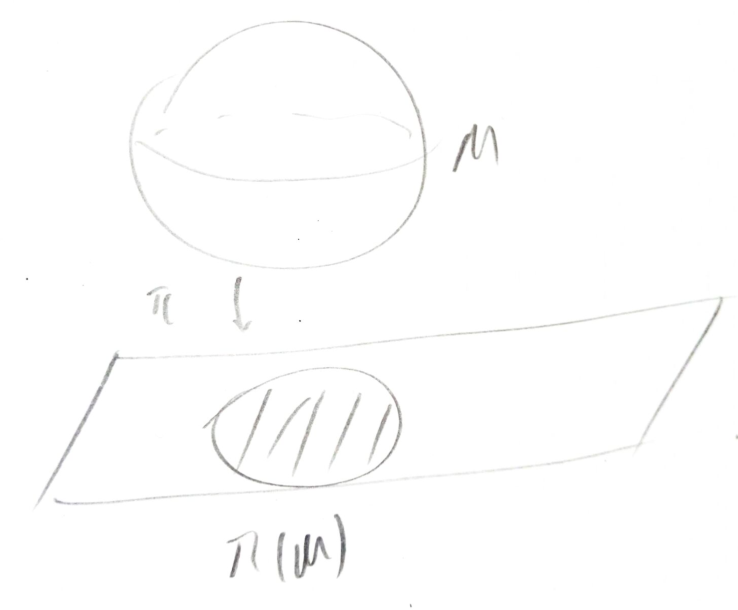
\includegraphics[width=0.8\textwidth]{sources/sphere-on-plane}
\caption{הטלת ספירה על המישור.}
\label{project:shpere-plane}
\end{figure}
\begin{description}
\item[חישוב \textenglish{I}:]
בקואורדינטות מקומיות ניקח
\begin{align*}
\Uu_1 = \set{\prs{x,y,z} \in S^1}{z>0}
\end{align*}
עם
\begin{align*}
\phi_1 \colon \Uu_1 &\to \RR^2 \\
\text{.} \phantom{\phi_1 \colon} \prs{x,y,z} &\to \prs{x,y}
\end{align*}
ראו איור
\ref{project:shpere-plane-map}
\begin{figure}[ht]
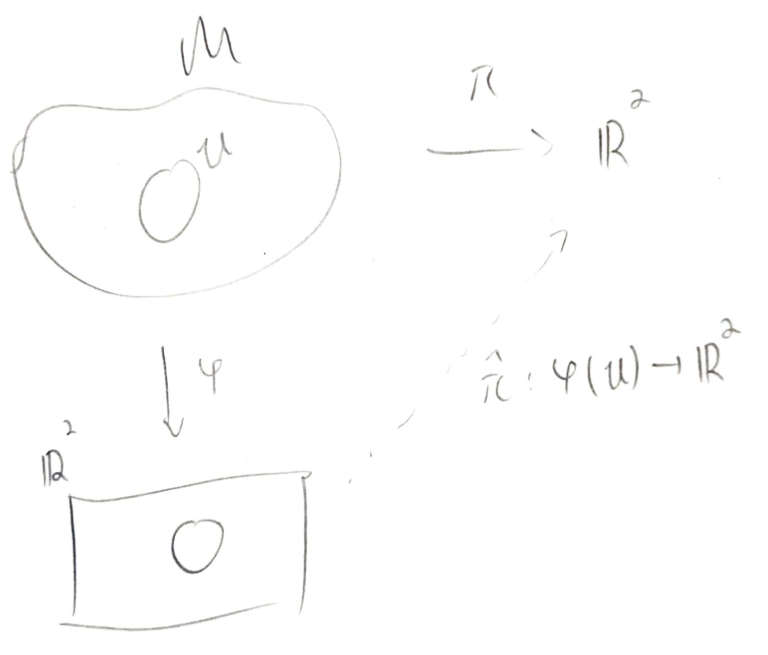
\includegraphics[width=0.8\textwidth]{sources/sphere-on-plane-map}
\caption{}
\label{project:shpere-plane-map}
\end{figure}
נחשב את ההעתקה המקומית.
\begin{align*}
\hat{\pi}_1 \colon \prs{x,y} \xrightarrow{\phi_1^{-1}} \prs{x,y,\sqrt{1-x^2-y^2}} \xrightarrow{\pi} \prs{x,y}
\end{align*}
לכן
$\hat{\pi}_1 = \1_{\phi_1\prs{\Uu_1}}$
ועל כן
$D\hat{\pi}_1 = I_2$.
נקבל כי
$\Uu_1$
נקודה רגולריות.
ניקח מפה נוספת
\begin{align*}
\Uu_2 &= \set{\prs{x,y,z}\in S^2}{x < 0} \\
\phi_2\prs{x,y,z} &= \prs{y,z}
\end{align*}
ואז
\[\hat{\pi}_2 \colon \prs{y,z} \xrightarrow{\phi_2^{-1}}\prs{\sqrt{1-y^2-z^2},y,z} \xrightarrow{\pi} \prs{-\sqrt{-y^2-z^2},y}\]
ולכן
\[D\hat{\pi}_2\prs{x,z} = \pmat{\frac{y}{\sqrt{\ldots}} & \frac{z}{\sqrt{\ldots}} \\ 1 & 0}\prs{y,z}\]
לא על אם ורק אם
$z=0$.
לכן הנקודות על קו המשווה חיתוך עם
$\Uu_2$
הן נקודות קריטיות.
עם נכסה את
$S^2$
במפות קואורדינטות, חישוב דומה יראה שהנקודות הקריטיות הן קו המשווה.
לכן הערכים הקריטיים יהיו מעגל היחידה.
\item[חישוב \textenglish{II}:]
נרחיב את
$\pi$
להעתקה
\begin{align*}
\pi \colon \RR^3 &\to \RR^2 \\
\prs{x,y,z} &\to \prs{x,y}
\end{align*}
ולכן
$\pi$
לינארית ונסמן
$\pi\prs{x} = Ax$.
אז
$D\pi = A$
ולכן
$\im D\pi\prs{x} = \RR^3$.
אז
$\ker D\pi\prs{x} = \mathrm{span}\prs{0}$.\\
$M \subseteq \RR^3$
משטח ולכן
$T_p M \subseteq T_p \RR^3 \cong \RR^3$
תת־מרחב דו מימדי.
נסמן
$\pi_M = \rest{\pi}{M} \colon M \to \RR^2$.
אז%
\footnote{מתקיים \begin{align*}
D\pi_M \colon TM &\to \RR^2 \\ \prs{p,u} &\to A\cdot u
\end{align*}
כאשר
$u \in T_pM$.}
\begin{align*}
\rest{D\pi}{T_p M} = D \pi_M\prs{p} \colon T_p M &\to \RR^2 \\
u &\to A\cdot u
\end{align*}
$D\pi_M\prs{p}$
לינארית ממרחב ממימד 2 למרחב ממימד 2 ולכן אינה על אם ורק אם
$\ker D\pi_M\prs{p} \neq \set{0}$.
נסמן
$v = \prs{0,0,1} = \ker D\pi$.
מתקיים
\begin{align*}
\ker D\pi_M\prs{p} = \ker \rest{D\pi\prs{p}}{T_pM} = \ker D\pi\prs{p} \cap T_p M = \set{\lambda \vec{v}}\cap T_p M
\end{align*}
לא טריוויאלי אם ורק אם
$\vec{v} \in T_p M$
אם ורק אם
$\vec{v}$
וקטור משיק ל־%
$M$
ב־%
$p$.
\end{description}
\end{example}
\begin{theorem}[\textenglish{Sard}]
תהי
$f \colon M^m \to N^n$
חלקה.
אז
$\set{y \in N}{\text{$y$ is a critical value}}$
קבוצה בעלת מידה אפס. (ביחס למידת לבג)
\end{theorem}
\begin{example}
\[\set{M \in M_{m\times n}\prs{\RR}}{\rank\prs{M} < \min\set{m,n}}\]
קבוצה בעלת מידה אפס.
\end{example}
\begin{proposition}
תהי
$C \in \RR^m$
זניחה ותהי
$f \colon \RR^m \to \RR^m$
חלקה. אז
$f\prs{C}$
זניחה.
\end{proposition}
\begin{corollary}
תהי
$M$
יריעה עם מפות
$\prs{\Uu, \phi}, \prs{\Vv, \psi}$
כאשר
$\Uu \cap \Vv \neq \ns$.
נקבל העתקה
\[\psi \circ \phi^{-1} \colon \phi\prs{\Uu} \to \psi\prs{\Vv}\]
חלקה.
לכן
$\phi \prs{C \cap \Uu \cap \Vv}$
זניחה ב־%
$\RR^m$
אם ורק אם
$\psi\prs{C \cap \Uu \cap \Vv}$
זניחה ב־%
$\RR^m$.
\end{corollary}
\begin{definition}
$C \subset M$
זניחה אם לכל מפה
$\prs{\Uu, \phi}$
מהאטלס החלק
$\phi\prs{C \cap \Uu}$
זניחה ב־%
$\RR^m$.
\end{definition}
\begin{example}
אם
$N^n \subseteq M^m$
ת־יריעה אז
$N$
זניחה ב־%
$M$.
\end{example}
\begin{example}
בהטלת
$S^2$
על
$\RR^2$
ראינו כי הערכים הקריטיים הם מעגל היחידה, וזאת קבוצה זניחה.
\end{example}
\begin{remark}
משפט
\text{Sard}
מתייחס ל%
\textbf{ערכים קריטיים}.
הטענה איננה נכונה עבור נקודות קריטיות.
עבןר ההעתקה
\begin{align*}
f \colon M &\to N \\
p &\to x_0 \in N
\end{align*}
כל נקודה ב־%
$M$
היא קריטית, ולכן לא זניחה.
\end{remark}
\begin{remark}
ייתכן כי
$\im\prs{f}$
מכילה רק ערכים קריטיים. במקרה זה
$\im\prs{f}$
זניחה ב־%
$N$.
\end{remark}
\begin{exercise}
בנו העתקה
$f \colon \RR \to \RR$
כל שקבוצת הערכים הקריטיים של
$f$
היא
$\QQ$.
\end{exercise}
\begin{corollary}
\begin{enumerate}
\item אם
$f \colon M \to N$
ו־%
$\dim M < \dim N$,
הערכים הקריטיים של
$f$
ב־%
$N$
זאת
$\im\prs{f}$.
אז
$\im\prs{f}$
בעלת מידה אפס.
\begin{example}
אין העתקה חלקה מ־%
$I \to I^2$
עם
$\im\prs{f} = I^2$.
\end{example}
\item קבוצת הערכים הרגולריים צפופה ב־%
$N$.
אם
$\Uu \subseteq \im\prs{f}$
פתוחה, קיים ערך רגולרי ב־%
$\im\prs{f}$.
\begin{example}
אם
$f \colon M \to \RR$
לא קבועה אז
$\prs{f\prs{x}, f\prs{y}} \subseteq \im\prs{f}$,
ויש ערך רגולרי ב־%
$\im\prs{f}$.
\end{example}
\end{enumerate}
\end{corollary}
\begin{proof}[\textenglish{Sard}]
נוכיח עבור המקרה
$\dim M \leq \dim N$.
המקרה הכללי בספר של
\textenglish{Milnor}.\\
נסמן ב־%
$C\subseteq M$
את קבוצת הנקודות הקריטיות של
$f$.
קבוצת הערכים הקריטיים היא
$f\prs{C} \subseteq N$.
נכסה את
$M$
על ידי מספר בן־מניה של מפות
$\prs{\Vv_i, \psi_i}$.
את
$f^{-1}\prs{\Vv_i}$
נכסה על ידי מספר בן־מניה של מפות
$\prs{\Uu_{i_j}, \phi_{i_j}}$
כך ש־%
$f\prs{\Uu_{i_j}} \subseteq \Vv_i$.
מתקיים
\begin{align*}
f\prs{C} = \bigcup_{i,j} f\prs{C \cap \Uu_{i_j}}
\end{align*}
ומספיק להראות כי
$f \prs{c \cap \Uu_{i_j}}$
זניחות.
מספיק להוכיח עבור הצגות מקומיות של
$f$.
כלומר, מספיק להוכיח את המשפט עבור
$f \colon \Uu\subseteq \RR^m \to \RR^n$.
$\Uu$
הינה איחוד בן־מניה של כדורים, לכן ניתן להניח ללא הגבלת הכלליות כי
$\Uu$
כדור עם סגור בתחום הגדרתה של
$f$.
\begin{enumerate}[label = \alph*.]
\item \textbf{המקרה $m=n$:}
נבחר
$\eps > 0$.
אז
$\abs{D f} \colon \bar{\Uu} \to \RR$
רציפה ולכן רציפה במ"ש.
לכן קיים
$\delta > 0$
כך שאם
$\norm{x-y} < \sqrt{m} \delta$
אז
$\abs{\abs{Df\prs{x}} - \abs{Df\prs{y}}} < \eps$.
יהי
$\Uu = \bigcup \Uu_i$
כיסוי על ידי קוביות על צלע
$\delta$
עם
$\sum \mrm{Vol} \Uu_i < 2^m \mrm{Vol}\prs{\Uu}$.
אם
$C \cap \Uu_i \neq \ns$,
קיימת
$x \in \Uu_i$
קריטית, כלומר
$\abs{D f\prs{x}} = 0$.
אז
$\abs{Df\prs{y}} < \eps$
לכל
$y \in \Uu_i$.
יהי
$I = \set{i}{\Uu_i \cap C \neq \ns}$.
אז
$\bigcup_{i\in I} f\prs{\Uu_i}$
כיסוי של
$f\prs{C}$.
כעת
\begin{align*}
\sum_{i\in I} \mrm{Vol}\prs{f\prs{\Uu_i}} &= \sum_{I} \int_{\Uu_i} \abs{Df\prs{x}} \diff x_1,\ldots,\diff x_m \\&\leq
\eps \sum_{i \in I} \mrm{Vol}\prs{\Uu_i} \leq \eps \mrm{Vol}\prs{\Uu}
\end{align*}
ולכן
$f\prs{C}$
זניחה.
\item \textbf{המקרה
$m < n$:}
תהי
$f \colon M^m \to N^n$
ונרחיב את
$f$
ל־%
$F \colon M^m \times \RR^{n-m} \to N^n$
ע"י
$F\prs{x,s} = f\prs{x}$.
אז קבוצת הערכים הקריטיים של
$f$
היא
$\im\prs{f}$.
גם
$\im\prs{f} = \im\prs{F}$.
לכן תמונת
$F$
היא קבוצת הערכים הקריטיים של
$f$.
קבוצה זאת זניחה לפי המקרה הקודם.
\end{enumerate}
\end{proof}

ראינו כי אם
$M^m$
יריעה קומפקטית, קיים שיכון
$M \xhookrightarrow{i} \RR^N$
עבור
$N$
גדול. ננסה להקטין את
$N$
בעזרת משפט
\textenglish{Sard}.
נרצה להטיל את
$i\prs{M}$
בכיוון
$v$
על
$v^{\perp}$
כך ש־%
$\pi_v \circ i \colon M \to v^{\perp}$
יהיה שיכון.
$M$
קומפקטית ולכן מספיק לבדוק כי זאת אימרסיה חד־חד ערכית.
\begin{description}
\item[אימרסיה:]
מתקיים כי
\[D\prs{\pi_v \circ i} = D\pi_v \circ D i\]
לכן
\[\text{.}\ker\prs{D\pi_v \circ D i} = \set{u}{Di\prs{u} \in \ker D\pi_v}\]
$Di$
חד־חד ערכית (כי
$i$
אימרסיה) לכן
$\ker D\pi_v \circ Di = \set{0}$
אם ורק אם
$\im D_i \cap \ker D\pi_v = \set{0}$.
מתקיים
$\ker D\pi_v = \set{\lambda v}{\lambda \in \RR}$.
אז
$\pi_v \circ i$
אימרסיה אם ורק אם
לכל
$x \in M$,
החיתוך
$\set{\lambda} \cap I_m Di\prs{x}$
טריוויאלי. זה שקול לכך שלכל
$x \in M$,
$v \notin \im Di\prs{x}$
($v$
אינו משיק ל־%
$i\prs{M}$
באף נקודה).
נגדיר העתקה
\[\text{.} g \colon TM \setminus M \times \set{0} \to \RR\P^{N-1}\]
גיאומטרית,
$\RR\P^{N-1}$
קבוצת הכיוונים האפשריים להטלה ב־%
$\RR^N$.
נגדיר
\[\text{.}\prs{x,u} \mapsto \brs{D i\prs{x}\prs{u}} = \set{\lambda Di\prs{x}\prs{u}}{\lambda \in \RR} \in \RR\P^{N-1}\]
אם
$\dim TM = 2m < N-1 = \dim \RR\P^{N-1}$,
לפי מסקנה ממשפט
\textenglish{Sard},
$\im g$
זניחה.
\item[חד־חד ערכיות:]
נגדיר העתקה
\begin{align*}
P \colon M\times M \setminus \Delta M &\to \RR\P^{N-1} \\
\prs{x,y} &\to \set{\lambda\prs{i\prs{x} - i\prs{y}}}{\lambda \in \RR}
\end{align*}
ואז כיוון בתמונה הוא בדיוק כיוון שאסור להטלה, כי זהו ישר המקביל לישר דרך
$i(x), i(y)$.
זה תנאי לזה ש־%
$\pi_v \circ i \prs{x} = \pi_v \circ i\prs{y}$
כלומר
$\pi_v \circ i$
לא חד־חד ערכית.
אם
$2m = \dim M\times M \setminus \Delta < \dim \RR\P^{N-1} = N-1$
נקבל כי
$\im P$
זניחה.
אז אם
$\set{\lambda v} \notin \im P \cup \im g$,
נקבל שיכון
$\pi_v \circ i \colon M \to v^{\perp} \cong \RR^{N-1}$.
זה מתקיים כמעט לכל
$v$
כי
$\im P \cup \im g$
זניחה.
התהליך נעצר כאשר
$2m = N-1$,
כלומר
$N = 2m + 1$.
\end{description}

\begin{remark}
המקרה האופטימלי הוא
$N = 2m$.
עם חישוב קצת יותר זהיר מקבלים ש־%
$\pi_v \circ i$
אימרסיה כמעט לכל
$v$
גם כאשר
$N = 2m + 1$,
כלומר ניתן לבנות אימרסיה
$M \to \RR^{2m}$.\\
אין דרך להבטיח חד־חד ערכיות באותו האופן.
ניתן להיפטר מנקודות חיתוך על ידי דיפורמציות טופולוגיות.
\end{remark}
\section{טרנסוורסליות}
\begin{definition}
יהי
$V$
מרחב וקטורי מעל
$\RR$
עם
$\dim V < \infty$.
תתי־מרחבים
$W_1,W_2 \leq V$
נקראים
\stress{טרנסוורסליים}
אם
$W_1 + W_2 = V$.
\end{definition}
\begin{remark}
$W_1,W_2$
טרנסוורסליים אם ורק אם
$\dim V = \dim W_1 + \dim W_2 - \dim\prs{W_1 \cap W_2}$
אם ורק אם
$\codim\prs{W_1 \cap W_2} = \codim W_1 + \codim W_2$.
\end{remark}
\begin{definition}
$M_1, M_2 \subseteq N$
תתי יריעות יקראו
\stress{טרנסוורסליות}
ונסמן
$M \pitchfork M_2$
אם לכל
$x \in M_1 \cap M_2$
מתקיים
$T_x M_1 + T_x M_2 = T_x N$.
\end{definition}
\begin{examples}
\begin{enumerate}
\item
אם
$\dim M_1 + \dim M_2 < \dim N$
אז
$M_1 \pitchfork M_2$
אם ורק אם
$M_1 \cap M_2 = \ns$.
\item
אם
$M_1, M_2 \subseteq \RR^2$
שני מעגלים נחתכים, סכום הישרים המשיקים בנקודות החיתוך הוא כל
$\RR^2$.
\item
אם
$M_1, M_2 \subseteq \RR^2$
שני מעגלים משיקים, בנקודת ההשקה סכום המרחבים המשיקים הוא
$\RR$,
ולכן המעגלים אינם טרנסוורסליים.
\end{enumerate}
\end{examples}
\begin{definition}
תהי
$f \colon M^m \to N^n$
חלקה ותהי
$L^l \subseteq N^n$
תת־יריעה.
נאמר כי
\stress{$f$
טרנסוורסלית ל־%
$L$}
ונסמן
$f \pitchfork L$
אם לכל
$p \in M$
עבורה
$f\prs{p} \in L$
מתקיים
$\im Df\prs{p} \pitchfork T_{f\prs{p}}L$.
\end{definition}
\begin{remark}
אם
$f$
שיכון,
$f \pitchfork L$
אם ורק אם
$\im f \pitchfork L$.
\end{remark}

ראינו כי עבור
$f \colon M \to N$
חלקה ו־%
$y \in N$
ערך רגולרי בתמונה,
$f^{-1}\prs{y}$
תת־יריעה של
$M$.
אנו רוצים להכליל זאת.

\begin{theorem}
תהי
$f \colon M \to N$
חלקה ו־%
$L$
תת־יריעה כך ש־%
$f \pitchfork L$
וגם
$\ns \neq f^{-1}\prs{L}$.
אזי
$f^{-1}\prs{L}$
תת־יריעה של
$M$
ומתקיים
\[\text{.}\codim_{M}\prs{f^{-1}\prs{L}} = \codim_N\prs{L}\]
\end{theorem}
\begin{exercise}
הוכיחו את המשפט.
\end{exercise}

\section{יריעות עם שפה}
\begin{definition}
תהי
$\hat{M}^m$
יריעה ותהי
$g \colon \hat{M} \to \RR$
חלקה עם
$0$
ערך רגולרי.
אז
$\set{g = 0} \subset \hat{M}$
תת־יריעה ממימד
$m-1$.
קבוצת הנקודות
$\set{x}{g\prs{x} \leq 0} \subseteq \hat{M}$
נקראת
\stress{יריעה עם שפה}.
\stress{השפה של $M$}
היא
\[\text{.} \del M \ceq \set{x}{g\prs{x} = 0}\]
\end{definition}
\begin{example}
ניקח
$\hat{M} = \RR^n$
ו־%
$g = \sum x_i^2 - 1$.
אז
$0$
ערך רגולרי ומתקיים
$\set{g \leq 0} = \overline{D^n}$
כדור היחידה הסגור.
מתקיים
$\del \overline{D^n} = S^{n-1}$.
\end{example}
\begin{example}
אינטרוול סגור, או אינטרוול חצי־פתוח חצי־סגור הם יריעות עם שפה.
\end{example}
\begin{remark}
קיבלנו מרחב שבו סביבת כל נקודה
$x$
הומאומורפית לקבוצה פתוחה ב־%
$\RR^n$
או לקבוצה פתוחה ב־%
$\RR^n_+ \ceq \set{\vec{x}}{x_n \geq 0}$.
ניתן להגדיר דרך סביבות אלה יריעה עם שפה בדומה להגדרת יריעה.
\end{remark}
\begin{definition}
תהיינה
$M$
יריעה עם שפה ו־%
$N$
יריעה.
$f \colon M \to N$
נקראת
\stress{חלקה}
אם ניתן להרחיב את
$f$
ל־%
$\hat{f} \colon \hat{M} \to N$
חלקה.
\end{definition}
\begin{definition}
$f \colon M \to N$
כאשר
$M,N$
יריעות עם שפה נקראת
\stress{חלקה}
אם
$f \colon M \to \hat{N}$
חלקה.
\end{definition}
\begin{exercise}[קשה]
תהי
$f \colon M^m \to N^n$
כאשר
$\del M \neq \ns$.
יהי
$y \in N$
ערך רגולרי של
$f$
ושל
$\rest{f}{\del M}$.
אז
$V = f^{-1}\prs{y}$
תת־יריעה עם שפה של
$M$
ומתקיים
$\dim V = m-n$
וגם
$\del V = V \cap \del M$.
\end{exercise}
\begin{definition}
יריעה
$M$
קומפקטית ללא שפה נקראת
\stress{סגורה}.
\end{definition}
\begin{remark}
תהי
$M$
יריעה עם שפה. אז
$\del M$
יריעה בלי שפה.%
\newlecture{18 באוקטובר}%
{2018}
כלומר
$\del \del M = \ns$.
\end{remark}
\begin{definition}
$M$
נקראת
\stress{יריעה עם פינות}
אם לכל
$x \in M$
קיימת מפה
$\prs{\Uu, \phi}$
עם
\[\text{,} \phi \colon \set{\vec{x} \in \RR^n}{\forall i \colon x_i \geq 0}\]
והאטלס מתואם.
\end{definition}
\begin{example}
קובייה
$I^n$
היא יריעה עם פינות.
\end{example}
\begin{example}
גופים פלטוניים הם יריעות עם פינות.
\end{example}
\begin{remark}
יריעה טופולוגית עם פינות היא בדיוק יריעה טופולוגית עם שפה.
אבל, בקטגוריה של יריעות חלקות, יריעה עם פינות איננה בהכרח יריעה עם שפה, אלא רק להפך.
\end{remark}
\section{הומוטופיה}
\section{הגדרות}
\begin{question}
תהיינה
$f,g\colon M \to N$
העתקות בין יריעות חלקות. מתי קיימת דפורמציה מ־%
$f$
ל־%
$g$?
\end{question}
\begin{definition}
$f$
\stress{הומוטופית}
ל־%
$g$
אם קיימת העתקה
$\Phi \colon M \times \brs{0,1} \to N$
חלקה המקיימת
\begin{align*}
\Phi\prs{x,0} &= f(x) \\
\text{.}\Phi\prs{x,1} &= g(x)
\end{align*}
\end{definition}
\begin{exercise}
הראו כי הומוטופיה בין העתקות היא יחס שקילות.
\end{exercise}
\begin{example}
כל
$f \colon M \to \RR^n$
הומוטופית ל־%
$g\prs{x} \equiv 0$.
נגדיר
$\Phi\prs{x,t} = t\cdot f\prs{x}$.
ראינו כי הומוטופיה הינה יחס שקילות, לכן כל שתי העתקות כאלו הומוטופיות.
\end{example}
\begin{example}
\label{homotopy: maps on sphere}
תהיינה
$M = N = S^n$
עם ההעתקות
\begin{align*}
\phi \colon S^n &\to S^n \\ x &\to x
\end{align*}
ו־%
\begin{align*}
\text{.}\psi \colon S^n &\to S^n \\ x &\to -x
\end{align*}
אז
$\phi,\psi$
עבור
$n$
זוגי,
ההעתקות אינן
הומוטופיות (נראה בהמשך).
\end{example}
\begin{definition}
\begin{align*}
v \colon M &\to TM \\ x &\to \prs{x,v_x}
\end{align*}
(כאשר כל
$v_x \in T_x M$)
נקרא
\stress{שדה וקטורי}.
הוא יקרא
\stress{חלק}
אם הוא חלק כהעתקה
$M \to TM$.
\end{definition}
\begin{example}
באינפי, הגדרנו שדה וקטורי להיות העתקה
$v \colon \RR^n \to \RR^n$.
בהגדרה שלנו
\begin{align*}
v \colon \RR^n &\to T\RR^n \\ x &\to \prs{x, v_x \in T_x\RR^n}
\end{align*}
כאשר
$T_x \RR^n \cong \RR^n$.
ניתן לתאר את
$v$
בעזרת העתקה
$x \to v_x \in \RR^n$.
\end{example}
תהיינה
$M$
יריעה, ו־%
$\prs{\Uu,\phi}$
מפה.
אז
\begin{align*}
D\phi \colon T\Uu &\xrightarrow{\sim} \phi\prs{\Uu}\times \RR^n \\
\rest{v}{\Uu} &\to \hat{v}
\end{align*}
הינו שדה וקטורי על
$\phi\prs{\Uu}$.
ההעתקה היא
\[\prs{x,v_x} \to \prs{\phi\prs{x},D\phi_x \cdot v_x}\]
ו־%
$v$
חלק אם ורק אם כל הצגה
$\hat{v}$
חלקה כפונקציה
$\phi\prs{\Uu} \to \RR^n$.

\begin{definition}
$v \colon M \to TM$
\stress{לא מנוון}
אם
$v_x \neq 0$
לכל
$x$.
\end{definition}
\begin{proposition}
נניח כי על
$S^n$
קיים שדה וקטורי לא מנוון. אז
$\phi, \psi$
מדוגמה
\ref{homotopy: maps on sphere}
הומוטופיות.
\end{proposition}
\begin{proof}
נבחר
$v$
לא־מנוון ונניח בה"כ כי
$\forall x \in S^n \colon \norm{v_x} = 1$.
נגדיר
\begin{align*}
\text{.}\Phi \colon S^n \times \brs{0,\pi} &\to S^n \\ \text{.}\prs{x,\theta} &\to x\cos\theta + v_x\sin\theta
\end{align*}
נסתכל על
$\mrm{Span}\prs{x,v_x} \subseteq \RR^{n+1}$
כמתואר באיור
%TODO fig 6.1
מתקיים
\begin{align*}
\trs{\Phi\prs{x,\theta},\Phi\prs{x,\theta}} &= \cancelto{1}{\norm{x}^2} \cos^2\theta + 2\cancelto{0}{\trs{x,v_x}}\cos\theta\sin\theta + \cancelto{1}{\norm{v_x}^2}\sin^2\theta = 1
\end{align*}
וגם
$\Phi\prs{x,0} = x = \phi\prs{x}$
ו־%
$\Phi\prs{x,\pi} = -x = \psi\prs{x}$,
לכן קיבלנו הומוטופיה כנדרש.
\end{proof}
\begin{theorem}
עבור
$n$
זוגי,
$\phi$
איננה הומוטופית ל־%
$\psi$.
\end{theorem}
\begin{proof}
\renewcommand{\blacksquare}{}
בעתיד.
\end{proof}
\begin{corollary}
על
$S^{2k}$
לא קיים שדה וקטורי לא מנוון. (אי־אפשר לסרק את הקיפוד)
\end{corollary}
\begin{corollary}
\[S^{2k} \times \RR^{2k} \not\cong TS^{2k}\]
כי עבור
$S^{2k} \times \RR^{2k}$
קיים שדה וקטורי לא מנוון.
\end{corollary}
\begin{example}
לכל
$n$
אי־זוגי מתקיים
$S^{2m+1} \subseteq \RR^{2m + 2} = \CC^{m+1}$.
לכל
$x = \prs{z_0, \ldots, z_m} \in S^{2m + 1}$
נגדיר
$v_x = \prs{iz_0, \ldots, iz_m} \perp x$
וקטור משיק. אז
$v \colon x \to ix$
שדה וקטורי לא מנוון ולכן
$\phi \cong \psi$.
\end{example}
\begin{theorem}
תהיינה
\begin{align*}
\phi \colon S^n &\to S^n \\ x &\to x
\end{align*}
\begin{align*}
\text{.}\psi \colon S^n &\to S^n \\ x &\to x_0
\end{align*}
אז
$\phi \not\sim\psi$.
\end{theorem}
\begin{proof}
בעתיד.
\renewcommand{\blacksquare}{}
\end{proof}
\begin{corollary}
תהי
$f \colon \bar{D}^{n+1} \to S^n$
חלקה.
אזי
$\rest{f}{S^n} \neq \1_{S^n}$.
כלומר, אין ריטרקציה חלקה מהדיסק לספירה.
\end{corollary}
\begin{remark}
נובע מכך עם אנליזה כי אין ריטרקציה רציפה מהדיסק לספירה.
\end{remark}
\begin{proof}
ניתן שתי הוכחות.
\begin{enumerate}
\item נניח בשלילה כי
$\rest{f}{S^n} = \1_{S^n}$.
נגדיר הומוטופיה
\begin{align*}
\Phi \colon S^n \times I &\to S^n \\
\prs{x,t} &\to f\prs{t\cdot x}
\end{align*}
ונקבל
$\Phi\prs{x,1} = f\prs{x} = x$
ו־%
$\Phi\prs{x,0} = f\prs{0} = \mrm{const}$
בסתירה למשפט.
\item
נניח בשלילה כי
$\rest{f}{S^n} = \1_{S^n}$.
יהי
$y \in S^n$
ערך רגולרי של
$f$
(קיים לפי
\textenglish{Sard}).
$y$
ערך רגולרי גם של
$\rest{f}{S^n} = \1_{S^n}$
(כל ערך הוא רגולרי של הזהות).
מתרגיל,
$L \ceq f^{-1}\prs{y}$
תת־יריעה עם שפה ממימד 1 ב־%
$\bar{D}^{n+1}$.
לכן, כל רכיב קשירות הוא
$S^1$
או
קטע.
כיוון ש־%
$f^{-1}\prs{y}$
קבוצה סגורה בקבוצה קומפקטית
$\bar{D}$,
היא קומפקטית בעצמה, ולכן כל הקטעים אם ישנם הינם סגורים.
בנוסף,
$\del L = f^{-1} \prs{y} \cap \del \bar{D}^{n+1} = \set{y}$
כי
$\1_{\del D} = \rest{f}{\del D}$.
זאת סתירה, כי ליריעה קומפקטית עם שפה יש מספר זוגי של נקודות שפה (קצוות של קטעים סגורים).
\end{enumerate}
\end{proof}
\begin{corollary}[משפט
\textenglish{Brouwer}]
לכל העתקה (חלקה)
$f \colon \bar{D}^n \to \bar{D}^n$
יש נקודות שבת.
\end{corollary}
\begin{proof}
נניח כי לכל
$x$
מתקיים
$f\prs{x} \neq x$.
נגדיר
\[\lambda_x = \set{f\prs{x} + t\prs{x - f\prs{x}}}{t > 0}\]
קרן שמתחילה ב־%
$f\prs{x}$
ועוברת דרך
$x$.
ראו איור
\ref{brouwer:map}.
\begin{figure}
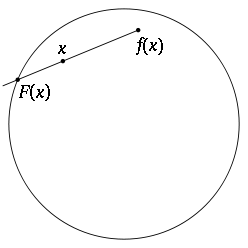
\includegraphics[scale=0.8]{sources/retraction_lemma}
\caption{העתקה למשפט בראואר.}
\label{brouwer:map}
\end{figure}
$\lambda_x$
חותכת את שפת הדיסק בנקודה אחת שנסמנה
$F(x)$.
אז
$F(x) = \lambda_x \cap \del D^n$.
$F$
חלקה (\stress{כתרגיל}), ואם
$x \in \del D^n$
אז
$F(x) = x$.
זאת סתירה למסקנה שאין רטרקציה מהדיסק לספירה.
\end{proof}
\begin{remark}
המשפט נכון גם עבור העתקות רציפות.
\end{remark}
\chapter{פיצול היחידה}
\begin{definition}
יהי
$\set{\Uu_{\alpha}}$
כיסוי של מרחב טופולוגי
$X$.
הכיסוי נקרא
\stress{סופי מקומית}
אם לכל
$x \in X$
קיימת סביבה
$\Ww$
כך ש־%
\[\#\set{\alpha}{\Ww \cap \Uu_{\alpha} \neq \ns}\]
סופי.
\end{definition}
\begin{definition}
יהי
$\set{\Vv_{\beta}}_{\beta}$
כיסוי של מרחב טופולוגי
$X$.
כיסוי
$\set{\Uu_{\alpha}}_{\alpha}$
\stress{עידון}
\textenglish{(refinement)}
של הכיסוי
$\set{\Vv_{\beta}}_{\beta}$
אם לכל
$\alpha$
קיים
$\beta$
עבורו
$\Uu_{\alpha} \subseteq \Vv_{\beta}$.
\end{definition}
\begin{definition}
מרחב
$X$
נקרא
\stress{פָרַקומפקטי} \textenglish{(paracompact)}
אם לכל כיסוי פתוח
$\set{\Uu_{\alpha}}_{\alpha}$
קיים עידון פתוח סופי מקומית.
\end{definition}
\begin{theorem}
כל יריעה טופולוגית האוסדורף בת־מנייה שנייה היא פָרַקומפקטית.
\end{theorem}
\begin{definition}
תהי
$M$
יריעה חלקה ותהי
$f \colon M \to \RR$
חלקה.
\stress{התומך} \textenglish{(support)}
של
$f$
הוא
\[\text{.} \mrm{supp}\prs{f} = \set{x\in M}{f(x) \neq 0}\]
\end{definition}
\begin{definition}
יהי
$\set{\Uu_{\alpha}}_{\alpha}$
כיסוי פתוח של יריעה
$M$.
\stress{פיצול יחידה} \textenglish{(partition of unity)}
הוא אוסף
$\Lambda$
של פונקציות חלקות
$\lambda_{\alpha} \colon M \to \brs{0,1}$
המקיימות את התנאים הבאים.
\begin{enumerate}
\item $\mrm{supp} \lambda_{\alpha} \subseteq \Uu_{\alpha}$
\item $\set{\mrm{supp} \lambda_{\alpha}}_{\alpha}$
כיסוי סופי מקומית.
\item לכל
$x \in M$
מתקיים
$\sum_{\alpha} \lambda_{\alpha}\prs{x} = 1$.\footnote{יש מספר סופי של מחוברים שונים מאפס, לכן הסכום סופי.}
\end{enumerate}
\end{definition}
\begin{remark}
פיצול היחידה תלוי בבחירת הכיסוי.
\end{remark}
\begin{theorem}
נניח כי
$M$
יריעה.
אז לכל כיסוי פתוח קיים פיצול יחידה.
\end{theorem}
\begin{proof}
נציג רק את רעיון ההוכחה.
ניקח כיסוי פתוח
$\set{\Uu_{\alpha}}_{\alpha}$.
נניח בה"כ כי
$\set{\Uu_{\alpha}}_{\alpha}$
סופי־מקומית.%
\footnote{
אחרת נחליף בעידון סופי מקומית%
}
נבחן כיסוי "קצת יותר עדין"
$\set{\Vv_{\alpha}}_{\alpha}$\footnote{קיים, אך דורש הוכחה}
כך ש־%
$\set{\Vv_{\alpha}}_{\alpha}$
כיסוי פתוח וגם
$\overline{V_{\alpha}} \subseteq \Uu_{\alpha}$.
נגדיר העתקה חלקה המקיימת
\begin{align*}
\Psi_{\alpha} \colon M &\to \brs{0,1} \\
x &\to \fcases{1 & x \in \overline{\Vv_{\alpha}} \\ 0 & \text{$x$ is in a small neighbourhood of $M \setminus \Uu_{\alpha}$}}
\end{align*}
זה קירוב של פונקציית האינדיקטור.
לכל
$x \in M$
קיים מספר סופי של
$\alpha$
כך ש־%
$\Psi_{\alpha}\prs{x} \neq 0$.
לכן
$\Psi\prs{x} \ceq \sum_{\alpha} \Psi_{\alpha}\prs{x}$.\footnote{מוגדר היטב, חיובית כי
$V_{\alpha}$
כיסוי}
נגדיר
$\lambda_{\alpha}\prs{x} = \frac{\Psi_{\alpha}\prs{x}}{\Psi\prs{x}}$.
אז
\[\mrm{supp}\prs{\lambda_{\alpha}} = \mrm{supp}\prs{\Psi_{\alpha}} \subseteq \Uu_{\alpha}\]
וגם
\[\text{.}\sum_{\alpha} \lambda_{\alpha}\prs{x} = \sum_{\alpha} \frac{\Psi_{\alpha}\prs{x}}{\Psi\prs{x}} = 1\]
$\set{\mrm{supp}\prs{\lambda_{\alpha}}}_{\alpha}$
כיסוי סופי מקומית כי זה נכון ל־%
$\set{\Uu_{\alpha}}_{\alpha}$.
\end{proof}

\section{מטריקה רימנית}

שימוש של
פיצול היחידה הוא הוכחה לכך שעל כל יריעה קיימת מטריקה רימנית.

\begin{definition}
\stress{מכפלה פנימית}
היא תבנית בילינארית סימטרית מוגדרת חיובית
$\rho \colon V\times V \to \RR$
כאשר
$V$
מרחב קטורי.
\end{definition}
\begin{definition}
תהי
$\Uu \subseteq \RR$
פתוחה.
\stress{מטריקה רימנית}
על
$\Uu$
היא משפחה חלקה של מכפלות פנימיות
$\rho_x \colon \RR^n \times \RR^n \to \RR$
שתלויות ב־%
$x \in \Uu$
באופן חלק.
\end{definition}
\begin{remark}
נחשוב על ההעתקות כעל העתקות
$\rho_x \colon T_x \RR^n \times T_x\RR^n \to \RR$.
\end{remark}
\begin{definition}
תהי
$M$
יריעה (חלקה).
\stress{מטריקה רימנית על
$M$}
היא בחירה חלקה של מכפלות פנימיות
$\rho_p \colon T_p M \times T_p M \to \RR$,
תלויה באופן חלק ב־%
$p$.
\end{definition}
\begin{remark}
$\rho_p$
חלקה אם ורק אם בקואורדינטות.
מתקבל מכפלה פנימית
\[\phi_{\alpha,*} \rho_p \colon T_{\phi\prs{p}}\RR^n \times T_{\phi\prs{p}}\RR^n \to \RR\]
ואז
\begin{align*}
\text{.} \hat{\rho}_{\alpha} = \phi_{\alpha, *}\rho_p\prs{v,w} = \rho_p \prs{D\phi_{\alpha}^{-1}\prs{p} v, D\phi_{\alpha}^{-1}\prs{p} w}
\end{align*}
\end{remark}
\begin{remark}
הדבר שקול לכך שלכל שני שדות וקטוריים חלקים
$v,w \colon M \to TM$,
$\rho\prs{V,W}$
פונקצייה חלקה
$M \to \RR$
עם ההגדרה
$\rho\prs{v,w}\prs{p} = \rho_p \prs{v_p, w_p}$.
\end{remark}

בעזרת מטריקה רימנית ניתן להגדיר אורך של וקטור משיק. אם
$v \in T_p M$
נגדיר
$\norm{v}_p^2 = \rho_p\prs{v,v}$
\stress{האורך של
$v$
ביחס למטריקה הרימנית
$\rho$}.

ניתן כך להגדיר גם אורך של מסילה
$\gamma \colon \brs{a,b} \to M$
על ידי
\[\text{.} \mrm{len}\prs{\gamma} \ceq \int_a^b \dot{\norm{\gamma}} \diff t\]

ניתן להגדיר זווית בין שני וקטורים משיקים
$u,v \in T_p M$
על ידי
\[\text{.} \rho_p\prs{u,v} = \norm{u} \norm{v} \cos \theta\]

\begin{theorem}
על כל יריעה יש מטריקה רימנית.
\end{theorem}
\begin{proof}
ב־%
$\RR^n$
ישנה מטריקה רימנית אוקלידית
\[\rho_0\prs{\vec{x},\vec{y}} = \trs{\vec{x},\vec{y}} = \sum_{i=1}^n x_i y_i\]
לכל נקודה
$p \in \RR^n$.
בהינתן מפה
$\prs{\Uu_{\alpha}, \phi_{\alpha}}$
נקבל
\[\rho_{\alpha} \ceq \phi_{\alpha}^* \rho_0 \prs{v, w} \ceq \rho_0 \prs{D \phi_{\alpha} v, D\phi_{\alpha} w}\]
מטריקה רימנית על
$\Uu_{\alpha}$.

נבחר כיסוי
$\set{\Uu_{\alpha}}_{\alpha}$
על ידי מפות מתואמות.
יהי
$\set{\lambda_{\alpha}}_{\alpha}$
פיצול היחידה המתאים ל־%
$\set{\Uu_{\alpha}}_{\alpha}$
ונגדיר
\[\bar{\rho}_{\alpha}(p) = \fcases{\lambda_{\alpha}\prs{p} \cdot \rho_{\alpha}\prs{p} & p \in \Uu_{\alpha} \\ 0 & p \in \Uu_{\alpha}}\]
תבנית חלקה.
אז
$\bar{\rho}\prs{p} = \sum_{\alpha} \bar{\rho}_{\alpha}\prs{p}$
תבנית חלקה (הסכום סופי מקומית), בילינארית סימטרית ומוגדרת חיובית כי
$\sum \lambda_{\alpha}\prs{p} = 1$
ולכן קיים
$\alpha$
עבורו
$\lambda_{\alpha}\prs{p} \neq 0$
והסכום אינו מנוון.
\end{proof}

נתאר הוכחה נוספת.

\begin{proof}
ממשפט
\textenglish{Whitney}
קיים שיכון
$i \colon M \hookrightarrow \RR^N$.
נגדיר
$i^* p \ceq \rho_0 \prs{Di\prs{p}\prs{v},Di\prs{p}\prs{w}}$
לכל
$v,w \in T_p M$,
מטריקה רימנית על
$M$.
\end{proof}
\begin{exercise}
תהי
$M \subseteq \RR^n$
תת־יריעה. ההגדרה של פונקציות חלקות
$M \to \RR^k$
בעזרת אטלס חלק שקולה להגדרה הבאה:
\\
$f \colon M \to \RR^k$
חלקה אם ורק אם ניתן למצוא סביבה
$\Uu$
של
$M$
ב־%
$\RR^n$
והרחבה חלקה
$f \colon \Uu \to \RR^k$.
\end{exercise}
\begin{exercise}
בדקו כי שתי ההגדרות שראינו ליריעה עם שפה שקולות.%
\footnote{מעבר מההגדרה הראשונה לשנייה מצריך את משפט הפונקציה הסתומה. הכיוון השני מצריך פיצול יחידה.}
\end{exercise}
\backmatter
\end{document}

